\documentclass[preprint,12pt]{elsarticle}

\usepackage[margin=2.3cm]{geometry}
\usepackage{amsmath,amssymb,bm}
\usepackage{mathtools}
\usepackage{graphicx}
\usepackage{booktabs}
\usepackage{multirow}
\usepackage{xcolor}
\usepackage[colorlinks=true,linkcolor=blue!55!black,citecolor=blue!55!black,urlcolor=blue!55!black]{hyperref}

\newcommand{\Tr}{\operatorname{Tr}}
\newcommand{\ket}[1]{\left|#1\right\rangle}
\newcommand{\bra}[1]{\left\langle#1\right|}
\newcommand{\braket}[2]{\left\langle#1\middle|#2\right\rangle}
\newcommand{\ketbra}[2]{\left|#1\right\rangle\!\left\langle#2\right|}
\newcommand{\dd}{\mathrm{d}}
\newcommand{\Erel}{E_{\rm rel}}
\newcommand{\Scl}{S_{\rm cl}}
\newcommand{\SW}{S_{W}}

\journal{Annals of Physics}

\begin{document}

\begin{frontmatter}

\title{Semiclassical entanglement of two coupled quantum rotors:\\
Bessel ladders, the separatrix, and phase-space distributions}

\author[a]{[Author list to be completed]}
\address[a]{[Affiliation]}

\begin{abstract}
For two rotors coupled by $\lambda\cos(\theta_{1}-\theta_{2})$ we compare the
entanglement entropy of highly excited eigenstates with the entropy of the
reduced classical microcanonical distribution, following the programme of
Duan, Kovner and Skokov for coupled oscillators, and we ask what changes when
the classical distribution is replaced by a quantum phase-space distribution.
Every sector of fixed total angular momentum is exactly a quantum pendulum
(Mathieu problem), and because the total angular momentum is conserved the
reduced density matrix is diagonal in the angular-momentum basis; the
phase-space cell is therefore fixed at $h$ and the comparison has no free
constant. Deep in the rotation regime the Schmidt weights are $J_{j}^{2}(\gamma)$,
$\gamma=\lambda I/\hbar^{2}n$, and the classical weights are the arcsine law; a
momentum-space WKB argument shows that the quantum entropy lies below the
classical one by $1-\ln2$, approached as $\gamma^{-1/3}$, and we confirm this to
$\gamma=10^{6}$. Both entropies are maximal near the separatrix, where the
support of the classical momentum distribution has a cusp, and in deep
libration $S_{0}=\tfrac14\ln(\lambda I/\hbar^{2})+\tfrac12\ln(\pi e/\sqrt2)
-[8\sqrt{2\lambda I/\hbar^{2}}\,]^{-1}+O(\hbar^{2}/\lambda I)$. Replacing the
classical distribution by the Wigner function reproduces the von Neumann
entropy identically, for every state and coupling: the Wigner function of the
reduced state is the marginal of the two-rotor Wigner function and equals the
Schmidt weights divided by $2\pi$. The constant $1-\ln2$ is the entropy carried
by the chord (interference) terms of the Wigner function, which survive the
marginalisation. With the Husimi function of the reduced state, the Wehrl
entropy exceeds the von Neumann entropy by $(1-\ln2)-D(\sigma)$, with $D$ given
in closed form and $D(\sigma)\simeq0.0802/\sigma$ for a coherent-state width
$\sigma\gtrsim1$, independently of $\gamma$. Quantum and classical
distributions smoothed by the same coherent state then agree to $O(1/\sigma)$ ---
at $\lambda I/\hbar^{2}=200$ and $800$, away from the separatrix, to $0.04$ for
$\sigma=1$ and $0.015$ for $\sigma=2$ --- but both entropies depend on
$\sigma$, which takes over the role of the arbitrary cell in the oscillator
problem.
\end{abstract}

\begin{keyword}
entanglement entropy \sep quantum rotors \sep quantum pendulum \sep
Wigner function \sep Husimi function \sep Wehrl entropy \sep
classical--quantum correspondence \sep separatrix
\end{keyword}

\end{frontmatter}

\tableofcontents
\newpage

%=============================================================================
\section{Introduction}
\label{sec:intro}
%=============================================================================

Duan, Kovner and Skokov (DKS)~\cite{DKS} asked how much of the entanglement of
a highly excited eigenstate is reproduced by a purely classical calculation.
For two coupled harmonic oscillators,
\begin{equation}
H_{c}=\tfrac12\left(p_{x}^{2}+p_{y}^{2}+\omega^{2}x^{2}+\Omega^{2}y^{2}
+2Cxy\right),\qquad C\ll\omega^{2}\ll\Omega^{2},
\label{eq:DKS}
\end{equation}
they integrated the microcanonical distribution over the second oscillator,
computed the Boltzmann entropy of the reduced distribution $W(x,p_{x})$, and
compared it with the von Neumann entropy of the reduced density matrix of a
WKB eigenstate. The two agree,
\begin{equation}
S_{\rm CE}=S_{E}=\ln\left[\frac{\pi C}{\Omega}
\frac{\sqrt{E_{1}E_{2}}}{\hbar\omega\Omega}\right],
\label{eq:DKSresult}
\end{equation}
provided the elementary phase-space cell used to make $W$ dimensionless is
$\Delta=h/2$; any other cell shifts the classical entropy by a constant. The
question is motivated by high-energy scattering, where the entanglement of the
probed degrees of freedom has been argued to become the Boltzmann entropy of
the final state~\cite{KharzeevLevin,Kutak,Hagiwara}.

The oscillator pair is Gaussian, has a non-compact phase space (so the cell is
not fixed by the theory), and has no separatrix. Two rotors on a circle,
\begin{equation}
H=\frac{p_{1}^{2}}{2I}+\frac{p_{2}^{2}}{2I}
+\lambda\cos\left(\theta_{1}-\theta_{2}\right),
\label{eq:H}
\end{equation}
remove all three restrictions at once while remaining solvable: the angular
momenta are quantised, which fixes the cell at $h$; the coupling is a cosine;
and the relative motion is a pendulum with a separatrix. In this paper we
treat the semiclassical regime, $\lambda I/\hbar^{2}\gg1$. The weak-coupling
regime, where the entropy is obtained in perturbation theory, is treated
separately~\cite{companion}; here it appears only as the small-$\gamma$ limit of
an exact solution (Sec.~\ref{sec:rotation}).

A natural alternative to the classical distribution is a quantum
quasi-probability distribution on phase space --- the Wigner
function~\cite{Hillery} or the Husimi function~\cite{Husimi} --- and
information measures built on these are an active subject in their own
right~\cite{Wehrl,PSinfo1,PSinfo2}. One may ask whether the DKS construction
works better, or differently, if the microcanonical distribution is replaced by
the Wigner or Husimi function of the eigenstate. The rotor pair answers this
question exactly, and the answer explains where the classical--quantum
difference comes from.

The results are the following.
\begin{enumerate}
\item Each sector of fixed total angular momentum is exactly a Mathieu problem,
and the entanglement entropy is the Shannon entropy of the Fourier
coefficients of a Mathieu function (Sec.~\ref{sec:model}). The reduced
classical distribution is obtained in closed form with an elliptic-integral
normalisation and a fixed cell $h$ (Sec.~\ref{sec:classical}).
\item In deep rotation the Schmidt weights are squared Bessel functions and the
classical weights the arcsine law; the quantum entropy lies below the
classical one by $1-\ln2$ in the semiclassical limit
(Sec.~\ref{sec:rotation}).
\item At generic energies the deficit grows towards the same constant; both
entropies are maximal near the separatrix (Sec.~\ref{sec:compare}).
\item In deep libration we obtain the ground-state entropy including the first
anharmonic correction (Sec.~\ref{sec:libration}).
\item The Wigner function of the reduced state is the marginal of the
two-rotor Wigner function and its entropy is the von Neumann entropy,
identically. The constant $1-\ln2$ is the entropy of the chord terms of the
Wigner function. The Husimi (Wehrl) entropy removes a fraction
$1-D(\sigma)/(1-\ln2)$ of the deficit, with $D$ in closed form, at the price of a
coherent-state width $\sigma$ that plays the role of the DKS cell
(Sec.~\ref{sec:wigner}).
\end{enumerate}
All calculations are given in full; standard integrals are collected in
\ref{app:integrals} and every analytic statement has been checked numerically
(\ref{app:num}).

%=============================================================================
\section{The model and its exact reduction}
\label{sec:model}
%=============================================================================

\subsection{Basis and conservation of total angular momentum}

Each rotor is described by an angle $\theta_{i}\in[0,2\pi)$ with
$p_{i}=-i\hbar\,\partial/\partial\theta_{i}$. Single-valuedness of
$e^{im\theta}$ requires $m\in\mathbb{Z}$, so $p_{i}=\hbar m_{i}$, and the
uncoupled basis is
\begin{equation}
\braket{\theta_{1},\theta_{2}}{m_{1},m_{2}}
=\frac{1}{2\pi}\,e^{im_{1}\theta_{1}}e^{im_{2}\theta_{2}},\qquad
H_{0}\ket{m_{1},m_{2}}=\frac{\hbar^{2}}{2I}\left(m_{1}^{2}+m_{2}^{2}\right)
\ket{m_{1},m_{2}} .
\label{eq:basis}
\end{equation}
Since $e^{\pm i\theta}\ket{m}=\ket{m\pm1}$ and
$\cos(\theta_{1}-\theta_{2})=\tfrac12[e^{i\theta_{1}}e^{-i\theta_{2}}+{\rm h.c.}]$,
\begin{equation}
\bra{m_{1}',m_{2}'}\cos(\theta_{1}-\theta_{2})\ket{m_{1},m_{2}}
=\frac12\left[\delta_{m_{1}',m_{1}+1}\delta_{m_{2}',m_{2}-1}
+\delta_{m_{1}',m_{1}-1}\delta_{m_{2}',m_{2}+1}\right]:
\label{eq:V}
\end{equation}
the coupling transfers one unit of angular momentum between the rotors. The
total angular momentum $J=p_{1}+p_{2}$ commutes with $H$, because
$(\partial_{\theta_{1}}+\partial_{\theta_{2}})\cos(\theta_{1}-\theta_{2})=0$, and
its eigenvalue $\hbar M$, $M=m_{1}+m_{2}$, labels invariant sectors
$\mathcal{H}_{M}$. Within a sector we use the relative label
\begin{equation}
k=\frac{m_{1}-m_{2}}{2}=m_{1}-\frac{M}{2},\qquad
m_{1}=\frac{M}{2}+k,\quad m_{2}=\frac{M}{2}-k,
\label{eq:k}
\end{equation}
which runs over $\mathbb{Z}$ for even $M$ and over $\mathbb{Z}+\tfrac12$ for
odd $M$. It is also convenient to write $n=2k=m_{1}-m_{2}$ and to introduce the
dimensionless coupling
\begin{equation}
\alpha=\frac{\lambda I}{2\hbar^{2}} .
\label{eq:alpha}
\end{equation}

\subsection{Centre-of-mass and relative variables}
\label{sec:cmrel}

Classically, introduce
\begin{equation}
\Theta=\frac{\theta_{1}+\theta_{2}}{2},\qquad
\varphi=\theta_{1}-\theta_{2},\qquad
J=p_{1}+p_{2},\qquad
p=\frac{p_{1}-p_{2}}{2}.
\label{eq:cmrel}
\end{equation}
The transformation is canonical, since
$p_{1}\dot\theta_{1}+p_{2}\dot\theta_{2}=J\dot\Theta+p\dot\varphi$. With
$p_{1}=J/2+p$, $p_{2}=J/2-p$ one has $p_{1}^{2}+p_{2}^{2}=J^{2}/2+2p^{2}$ and
\begin{equation}
H=\frac{J^{2}}{4I}+\underbrace{\frac{p^{2}}{I}+\lambda\cos\varphi}_{H_{\rm rel}} .
\label{eq:Hcm}
\end{equation}
The relative motion is a pendulum with moment of inertia $\mu=I/2$. Its
potential has a minimum $-\lambda$ at $\varphi=\pi$ and a maximum $+\lambda$ at
$\varphi=0$, so the separatrix is at
\begin{equation}
\Erel\equiv E-\frac{J^{2}}{4I}=\lambda .
\label{eq:separatrix}
\end{equation}
For $|\Erel|<\lambda$ the relative angle librates about $\varphi=\pi$; for
$\Erel>\lambda$ it circulates. Quantum mechanically $J=\hbar M$ and $p=\hbar k$.

\subsection{Each sector is a quantum pendulum}
\label{sec:pendulum}

Completing the square, $m_{1}^{2}+m_{2}^{2}=M^{2}/2+2k^{2}$, so by
\eqref{eq:basis} and \eqref{eq:V}
\begin{equation}
H\big|_{\mathcal{H}_{M}}=\frac{\hbar^{2}M^{2}}{4I}+h,\qquad
h_{kk'}=\frac{\hbar^{2}}{I}k^{2}\,\delta_{kk'}
+\frac{\lambda}{2}\left(\delta_{k',k+1}+\delta_{k',k-1}\right),
\label{eq:hsector}
\end{equation}
a real symmetric tridiagonal matrix. In sector $M$ the wave function
factorises,
$e^{im_{1}\theta_{1}+im_{2}\theta_{2}}=e^{iM\Theta}e^{ik\varphi}$, so
$\Psi=e^{iM\Theta}u(\varphi)/\sqrt{2\pi}$ with
$u(\varphi)=\sum_{k}c_{k}\,\chi_{k}(\varphi)$, $\chi_{k}=e^{ik\varphi}/\sqrt{2\pi}$.
The operator
\begin{equation}
h=-\frac{\hbar^{2}}{I}\frac{\dd^{2}}{\dd\varphi^{2}}+\lambda\cos\varphi
\label{eq:mathieuop}
\end{equation}
has exactly the matrix \eqref{eq:hsector} in the basis $\chi_{k}$, since
$\lambda\cos\varphi\,\chi_{k}=\tfrac{\lambda}{2}(\chi_{k+1}+\chi_{k-1})$. Each
sector is therefore the quantum pendulum $H_{\rm rel}$ of \eqref{eq:Hcm}, with
periodic boundary conditions for even $M$ and antiperiodic ones for odd $M$.
With $\varphi=2z$ the eigenvalue equation $hu=\Erel u$ becomes the Mathieu
equation~\cite{DLMF28,AbramowitzStegun}
\begin{equation}
\frac{\dd^{2}u}{\dd z^{2}}+\left(a-2q\cos2z\right)u=0,\qquad
a=\frac{4I\Erel}{\hbar^{2}},\qquad q=\frac{2\lambda I}{\hbar^{2}}=4\alpha,
\label{eq:mathieu}
\end{equation}
and
\begin{equation}
E=\frac{\hbar^{2}M^{2}}{4I}+\frac{\hbar^{2}}{4I}\times
\begin{cases}a_{0}<b_{2}<a_{2}<b_{4}<\dots, & M\ \text{even},\\[2pt]
b_{1}<a_{1}<b_{3}<a_{3}<\dots, & M\ \text{odd},\end{cases}
\label{eq:Emathieu}
\end{equation}
which we have checked to all printed digits against exact diagonalisation
(Table~\ref{tab:checks}). The separatrix is at $a=2q$. The Bohr--Sommerfeld
area inside the separatrix,
\begin{equation}
\oint p\,\dd\varphi=2\sqrt{2I\lambda}\int_{0}^{2\pi}\sin\frac{\varphi}{2}\,\dd\varphi
=8\sqrt{2I\lambda},
\end{equation}
gives the number of librating levels
\begin{equation}
N_{\rm lib}\simeq\frac{8\sqrt{2I\lambda}}{2\pi\hbar}=\frac{4}{\pi}\sqrt{q};
\end{equation}
for $\lambda I/\hbar^{2}=50,200,800,3200$ this is $12.7,25.5,50.9,101.9$,
against $13,25,51,102$ counted.

\subsection{The entanglement entropy is a Shannon entropy}
\label{sec:S}

The reduced density matrix of rotor 1 is
$\rho_{1}=\Tr_{2}\rho=\sum_{m}\bra{m}_{2}\rho\ket{m}_{2}$, and on a single dyad
\begin{equation}
\Tr_{2}\ketbra{a,b}{c,d}=\delta_{bd}\,\ketbra ac .
\label{eq:ptrace}
\end{equation}
An eigenstate in sector $M$ is
$\ket\Psi=\sum_{k}c_{k}\ket{\tfrac{M}{2}+k,\tfrac{M}{2}-k}$. Two different
values of $k$ carry different rotor-2 labels, so by \eqref{eq:ptrace} every
cross term drops out:
\begin{equation}
\rho_{1}=\sum_{k}|c_{k}|^{2}\,\ketbra{\tfrac{M}{2}+k}{\tfrac{M}{2}+k},
\qquad
\boxed{\;S_{q}=-\sum_{k}p_{k}\ln p_{k},\qquad p_{k}=|c_{k}|^{2}\;}
\label{eq:Smathieu}
\end{equation}
exactly. The entanglement entropy is the Shannon entropy of the Fourier
coefficients of a Mathieu function. Conservation of $J$ fixes the Schmidt basis
to be the angular-momentum basis, whatever the energy and the coupling; this
fact will be decisive in Secs.~\ref{sec:rotation} and \ref{sec:wigner}.

\subsection{Exchange symmetry, doublets and branch states}
\label{sec:ln2}

The exchange $P:\theta_{1}\leftrightarrow\theta_{2}$ maps $k\to-k$ and commutes
with $H$; in the Mathieu language it is $z\to-z$, with $\mathrm{ce}$ and
$\mathrm{se}$ its even and odd eigenfunctions, so every exact eigenstate has
$c_{-k}=\pm c_{k}$. Above the separatrix the levels form doublets of opposite
parity, split by an amount that vanishes as $\lambda^{|n|}$ at weak coupling
and exponentially in the semiclassical regime: the two members are the even and
odd combinations of two \emph{branch} states $\ket{\Psi_{\pm n}}$ describing
relative rotation in the two senses, $\ket{\Psi_{-n}}=P\ket{\Psi_{n}}$. On
times short compared with the inverse splitting a branch state is effectively
stationary.

If the branch weights $q_{k}=|\braket{k}{\Psi_{n}}|^{2}$ are supported on
$k>0$ (up to exponentially small tails), the parity eigenstate
$(\ket{\Psi_{n}}\pm\ket{\Psi_{-n}})/\sqrt2$ has $p_{\pm k}=q_{k}/2$ and, by
\eqref{eq:Smathieu},
\begin{equation}
S_{\rm exact}=-2\sum_{k>0}\frac{q_{k}}{2}\ln\frac{q_{k}}{2}
=\ln2+S_{\rm branch}.
\label{eq:Sln2}
\end{equation}
Note that no cross term can contribute, because $\rho_{1}$ is diagonal; only
the overlap of the two supports could. Classically the two branches are the
two invariant tori $p>0$ and $p<0$ of the level set, which the microcanonical
distribution weights equally (Sec.~\ref{sec:classical}), so the same $\ln2$
appears on both sides. Below the separatrix there is one torus and the levels
are non-degenerate.

\subsection{Parity sectors in the plane-wave basis}
\label{sec:parity}

Because the doublets are exponentially close, a dense eigensolver applied to
\eqref{eq:hsector} returns arbitrary mixtures of their members. We diagonalise
in the eigenspaces of $P$ separately. For even $M$ the even sector has basis
$\{\chi_{0},(\chi_{k}+\chi_{-k})/\sqrt2\}_{k\ge1}$, in which
$\bra{\chi_{0}}h\,\tfrac{1}{\sqrt2}(\chi_{1}+\chi_{-1})\rangle=\lambda/\sqrt2$
while all other off-diagonal elements are $\lambda/2$; the odd sector has basis
$\{(\chi_{k}-\chi_{-k})/\sqrt2\}_{k\ge1}$ with off-diagonal elements
$\lambda/2$. Every even-$M$ sector is identical to $M=0$ up to the constant
$\hbar^{2}M^{2}/4I$, and every odd-$M$ sector to $M=1$; all numerics below use
$M=0$ and $\hbar=I=1$.

%=============================================================================
\section{The classical reduced distribution}
\label{sec:classical}
%=============================================================================

\subsection{Microcanonical distribution and its marginal}

Following~\cite{DKS}, the classical counterpart of an eigenstate with definite
energy and total angular momentum is the microcanonical distribution on the
corresponding level set,
\begin{equation}
W_{\rm cl}(\theta_{1},p_{1};\theta_{2},p_{2})=\mathcal{C}\;
\delta\!\left(E-H\right)\,\delta\!\left(J-p_{1}-p_{2}\right),
\label{eq:Wjoint}
\end{equation}
normalised to one. It is invariant under the flow and uniform in the angle
variables of each invariant torus. For $\Erel>\lambda$ the level set consists of
two tori ($p>0$ and $p<0$) of equal weight; for $|\Erel|<\lambda$ of one.

The reduced distribution of rotor 1 is $W_{\rm cl}(\theta_{1},p_{1})=\int\dd\theta_{2}
\dd p_{2}\,W_{\rm cl}$. The second delta function sets $p_{2}=J-p_{1}$, after
which, with $p=p_{1}-J/2$ and $\varphi=\theta_{1}-\theta_{2}$,
\begin{equation}
W_{\rm cl}(\theta_{1},p_{1})=\mathcal{C}\int_{0}^{2\pi}\dd\varphi\;
\delta\!\left(\Erel-\frac{p^{2}}{I}-\lambda\cos\varphi\right).
\end{equation}
The argument vanishes at $\cos\varphi=\xi\equiv(\Erel-p^{2}/I)/\lambda$, i.e.\ at
the two angles $\varphi=\pm\arccos\xi$ when $|\xi|<1$, where the derivative has
modulus $\lambda\sqrt{1-\xi^{2}}$. Hence
\begin{equation}
\boxed{\;
W_{\rm cl}(\theta_{1},p_{1})=\frac{2\mathcal{C}}
{\sqrt{\lambda^{2}-\left(\Erel-p^{2}/I\right)^{2}}}\;
\Theta\!\left(\lambda-\left|\Erel-p^{2}/I\right|\right)\;}
\label{eq:Wclass}
\end{equation}
independent of $\theta_{1}$. The two roots $\varphi=\pm\arccos\xi$ --- two
relative angles compatible with one momentum of rotor 1 --- are the two
classical branches whose quantum interference is the subject of
Secs.~\ref{sec:rotation} and \ref{sec:wigner}.

\subsection{The support and its cusp at the separatrix}

The band $|\Erel-p^{2}/I|\le\lambda$ is $|p|\le\sqrt{I(\Erel+\lambda)}$ in
libration and $\sqrt{I(\Erel-\lambda)}\le|p|\le\sqrt{I(\Erel+\lambda)}$ in
rotation, of total length
\begin{equation}
L(\Erel)=\begin{cases}2\sqrt{I(\Erel+\lambda)}, & \Erel<\lambda,\\[2pt]
2\left[\sqrt{I(\Erel+\lambda)}-\sqrt{I(\Erel-\lambda)}\right], & \Erel>\lambda .
\end{cases}
\label{eq:support}
\end{equation}
$L$ increases through libration, reaches its maximum $2\sqrt{2I\lambda}$ at the
separatrix and decreases above it with $\dd L/\dd\Erel\to-\infty$ as
$\Erel\to\lambda^{+}$: a cusp maximum. Since the entropy of a distribution on
a set of length $L$ is at most $\ln(L/\hbar)$, this is the origin of the
entropy maximum of Sec.~\ref{sec:compare}.

\subsection{Normalisation and the classical period}

The momentum density is $w(p_{1})=2\pi W_{\rm cl}$. Its normalisation needs
the band integral
$B(\Erel)=\int_{{\rm band},\,p>0}\dd p\,[\lambda^{2}-(\Erel-p^{2}/I)^{2}]^{-1/2}$.
With $\Erel-p^{2}/I=\lambda\cos u$, $B=\tfrac{\sqrt I}{2}\int\dd u\,
(\Erel-\lambda\cos u)^{-1/2}$, and the standard substitutions give
(\ref{app:integrals})
\begin{equation}
B=\begin{cases}
\sqrt{\dfrac{I}{\Erel+\lambda}}\;\mathsf{K}(k),\quad
k^{2}=\dfrac{2\lambda}{\Erel+\lambda}, & \Erel>\lambda,\\[10pt]
\sqrt{\dfrac{I}{2\lambda}}\;\mathsf{K}(\kappa),\quad
\kappa^{2}=\dfrac{\Erel+\lambda}{2\lambda}, & |\Erel|<\lambda,
\end{cases}
\label{eq:B}
\end{equation}
with $\mathsf{K}$ the complete elliptic integral of the first kind. In either
regime the total weight is $2B$, so
\begin{equation}
\mathcal{C}=\frac{1}{8\pi B},\qquad
w(p_{1})=\frac{1}{2B}\,\frac{1}{\sqrt{\lambda^{2}-(\Erel-p^{2}/I)^{2}}}.
\label{eq:wnorm}
\end{equation}
With $\dot\varphi=2p/I$ the same substitution shows that the period of the
relative motion is $T=2B$: $w(p_{1})\,\dd p_{1}$ is the fraction of the period
spent in $\dd p_{1}$. At the separatrix $\mathsf{K}$ diverges logarithmically.

\subsection{Boltzmann entropy and the elementary cell}
\label{sec:cell}

The Boltzmann entropy of the reduced distribution,
$\Scl=-\int\dd\theta_{1}\dd p_{1}\,W_{\rm cl}\ln(W_{\rm cl}\Delta)$, requires a
cell $\Delta$. On a compact configuration space $\Delta$ is not free:
$p_{1}=\hbar m_{1}$, and each quantum state occupies the strip
$2\pi\times\hbar=h$. With $\Delta=h$ and $W_{\rm cl}=w/2\pi$,
\begin{equation}
\Scl=-\int\dd p_{1}\;w\ln\left(w\hbar\right),
\label{eq:Sdiff}
\end{equation}
a differential entropy in units of $\hbar$. The object with the same status as
\eqref{eq:Smathieu} is the Shannon entropy of the cell weights,
\begin{equation}
w_{m}=\int_{\hbar(m-1/2)}^{\hbar(m+1/2)}w(p_{1})\,\dd p_{1},\qquad
\Scl^{\rm bin}=-\sum_{m}w_{m}\ln w_{m}.
\label{eq:Sbin}
\end{equation}
The comparison between \eqref{eq:Sbin} and \eqref{eq:Smathieu} contains no
adjustable constant. Writing $\varrho=w/w_{m}$ on cell $m$,
\begin{equation}
\Scl=\Scl^{\rm bin}-\sum_{m}w_{m}\,D_{\rm KL}\!\left(\varrho\,\Vert\,
\hbar^{-1}\right)\le\Scl^{\rm bin},
\end{equation}
with $D_{\rm KL}$ the relative entropy with respect to the uniform density on
the cell. The difference comes from the cells that contain the
inverse-square-root singularities at the band edges and decreases as
(band width in cells)$^{-1/2}$.

%=============================================================================
\section{Deep rotation: an exactly solvable limit and the constant $1-\ln2$}
\label{sec:rotation}
%=============================================================================

\subsection{Reduction to a Wannier--Stark ladder}

Consider a level with large relative angular momentum, $k_{0}=n/2\gg1$, and
write $k=k_{0}+j$. Then
\begin{equation}
\frac{\hbar^{2}}{I}k^{2}=\frac{\hbar^{2}}{I}k_{0}^{2}+F\,j+\frac{\hbar^{2}}{I}j^{2},
\qquad F\equiv\frac{2\hbar^{2}k_{0}}{I}=\frac{\hbar^{2}n}{I}.
\end{equation}
For $|j|\lesssim\gamma$ (defined below) the quadratic term is smaller than the
linear one by $|j|/n\le\gamma/n$. Dropping it, \eqref{eq:hsector} becomes, up to
a constant,
\begin{equation}
h_{\rm WS}\,c_{j}=F\,j\,c_{j}+\frac{\lambda}{2}\left(c_{j+1}+c_{j-1}\right),
\label{eq:WS}
\end{equation}
a particle hopping on a lattice in a uniform field: the Wannier--Stark
problem~\cite{Wannier,Fukuyama}. Try $c_{j}=J_{j-s}(x)$ with $s\in\mathbb{Z}$.
The recurrence $J_{\nu-1}(x)+J_{\nu+1}(x)=(2\nu/x)J_{\nu}(x)$ gives
\begin{equation}
\frac{\lambda}{2}\left(c_{j+1}+c_{j-1}\right)
=\frac{\lambda(j-s)}{x}c_{j},\qquad
h_{\rm WS}c_{j}=\left[Fj+\frac{\lambda(j-s)}{x}\right]c_{j},
\end{equation}
which is independent of $j$ if and only if $x=-\lambda/F$; the eigenvalue is
then $Fs$. Using $J_{\nu}(-x)=(-1)^{\nu}J_{\nu}(x)$,
\begin{equation}
|c_{j}|^{2}=J_{j-s}^{2}(\gamma),\qquad
\boxed{\;\gamma\equiv\frac{\lambda}{F}=\frac{\lambda I}{\hbar^{2}n}
=\frac{2\alpha}{n}\;}
\label{eq:bessel}
\end{equation}
normalised by the Neumann identity $\sum_{j}J_{j}^{2}(\gamma)=1$. The
eigenvectors are translates of one another, so all have the same entropy. The
neglected term is small when $\gamma/n=\lambda/4\Erel\ll1$, deep in the
rotation regime. Exact diagonalisation confirms \eqref{eq:bessel} pointwise to
$3\times10^{-3}$ at $\gamma=2,5$ ($\gamma/n=0.01$) and the entropy to four or
five digits for $n=100$--$400$ (Fig.~\ref{fig:rotation}a).

The Bessel eigenvector is a branch state: it is centred on $k_{0}>0$ and its
weight on $k<0$ is negligible, so the parity eigenstate has entropy
$\ln2+S_{\rm branch}$ by \eqref{eq:Sln2}.

\subsection{The branch entropy as a function of one variable}

From \eqref{eq:Smathieu} and \eqref{eq:bessel} the branch entropy in deep
rotation is a universal function of $\gamma$ alone,
\begin{equation}
\boxed{\;S_{\rm branch}(\gamma)=-\sum_{j\in\mathbb{Z}}J_{j}^{2}(\gamma)\ln
J_{j}^{2}(\gamma)\;}
\label{eq:SB}
\end{equation}
\emph{Small $\gamma$.} With $J_{0}^{2}=1-\gamma^{2}/2+\dots$ and
$J_{\pm1}^{2}=\gamma^{2}/4+\dots$,
\begin{equation}
S_{\rm branch}\simeq2\cdot\frac{\gamma^{2}}{4}\ln\frac{4}{\gamma^{2}}
+\frac{\gamma^{2}}{2}=\gamma^{2}\left[\ln\frac{2}{\gamma}+\frac12\right].
\label{eq:Ssmall}
\end{equation}
This is second-order perturbation theory in $\lambda$: $\gamma^{2}/4$ is the
weight transferred to each neighbour $n\pm2$, and the term $\gamma^{2}/2$ comes
from the depletion $1-\gamma^{2}/2$ of the unperturbed component, i.e.\ from the
$O(\lambda^{2})$ normalisation of the perturbed state, which must be kept in the
density matrix~\cite{companion}.

\emph{Large $\gamma$.} The weights become many and the classical description
applies; we treat this next.

\subsection{The classical counterpart: the arcsine law}

In the same limit, linearising $p^{2}/I$ about $p_{0}=\sqrt{I\Erel}=\hbar n/2$
in \eqref{eq:Wclass} gives
$w\propto[a^{2}-(p-p_{0})^{2}]^{-1/2}$ with half-width $a=I\lambda/2p_{0}$,
i.e.\ $a/\hbar=\gamma$. The classical weights are the arcsine law,
\begin{equation}
w(j)=\frac{1}{\pi\sqrt{\gamma^{2}-j^{2}}},\qquad |j|<\gamma,
\label{eq:arcsine}
\end{equation}
whose differential entropy is (\ref{app:integrals})
\begin{equation}
\Scl^{\,\rm branch}=\ln\frac{\pi\gamma}{2},\qquad
\Scl^{\,\rm two\ bands}=\ln(\pi\gamma)
=\ln\left[\frac{\pi\lambda}{2\hbar}\sqrt{\frac{I}{\Erel}}\,\right].
\label{eq:Sclrot}
\end{equation}
This is the rotor counterpart of \eqref{eq:DKSresult}: the entropy grows
logarithmically with the coupling and decreases logarithmically with the
relative energy.

\subsection{Interference fringes in the quantum weights}

The quantum weights oscillate about the arcsine law. The Debye expansion of the
Bessel function~\cite{DLMF10}, with $j=\gamma\cos\beta$, $0<\beta<\pi$, reads
$J_{j}(\gamma)\simeq\sqrt{2/(\pi\gamma\sin\beta)}\,
\cos(\gamma\sin\beta-j\beta-\pi/4)$. Squaring,
\begin{equation}
J_{j}^{2}(\gamma)\simeq w(j)\left[1+\cos\Phi_{j}\right],\qquad
\Phi_{j}=2\sqrt{\gamma^{2}-j^{2}}-2j\arccos\frac{j}{\gamma}-\frac{\pi}{2},
\label{eq:fringes}
\end{equation}
fringes of \emph{full} contrast about the classical weights. Their local
wavenumber is
\begin{equation}
\frac{\dd\Phi_{j}}{\dd j}=-\frac{2j}{\sqrt{\gamma^{2}-j^{2}}}
-2\arccos\frac{j}{\gamma}+\frac{2j}{\sqrt{\gamma^{2}-j^{2}}}=-2\beta,
\label{eq:wavenumber}
\end{equation}
ranging over $(-2\pi,0)$ across the band.

The same structure holds at any energy. In the $k$ representation the
eigenvalue equation is the difference equation
$\frac{\hbar^{2}}{I}k^{2}c_{k}+\frac{\lambda}{2}(c_{k+1}+c_{k-1})=\Erel c_{k}$.
The WKB ansatz $c_{k}=A_{k}e^{i\chi_{k}}$ with slowly varying $A_{k}$ and local
wavenumber $\phi_{k}=\chi_{k+1}-\chi_{k}$ gives at leading order
$\Erel-\hbar^{2}k^{2}/I=\lambda\cos\phi_{k}$: the local wavenumber is the
classical relative angle at momentum $\hbar k$, and the two roots $\pm\phi_{k}$
are the two branches of \eqref{eq:Wclass}. The Casoratian
$\tfrac{\lambda}{2}(c_{k}\bar c_{k+1}-c_{k+1}\bar c_{k})$ of two solutions is
independent of $k$, which for one WKB wave gives
$|A_{k}|^{2}\lambda\sin\phi_{k}={\rm const}$, i.e.\
$|A_{k}|^{2}\propto[\lambda^{2}-(\Erel-\hbar^{2}k^{2}/I)^{2}]^{-1/2}$: the
classical density. A real eigenvector superposes the two waves with equal
amplitude, so
\begin{equation}
p_{k}\simeq w_{k}\left(1+\cos\Phi_{k}\right),\qquad
\Phi_{k+1}-\Phi_{k}=2\phi_{k}.
\label{eq:fringesgen}
\end{equation}
The classical distribution is the fringe average of the quantum one.

\subsection{The entropy deficit}

Insert \eqref{eq:fringesgen} into \eqref{eq:Smathieu}:
\begin{equation}
S_{q}=\Scl^{\rm bin}-\sum_{k}w_{k}\cos\Phi_{k}\ln w_{k}
-\sum_{k}w_{k}(1+\cos\Phi_{k})\ln(1+\cos\Phi_{k}).
\end{equation}
In the second term $\cos\Phi_{k}$ oscillates on the scale of a few cells while
$w_{k}\ln w_{k}$ varies on the scale of the band, so it vanishes as the band
widens. In the third the phases $\Phi_{k}\bmod2\pi$ are equidistributed wherever
$2\phi_{k}$ is not close to a multiple of $2\pi$, and the sum becomes a phase
average (\ref{app:integrals}):
\begin{equation}
\Scl-S_{q}\;\longrightarrow\;\frac{1}{2\pi}\int_{0}^{2\pi}
(1+\cos\Phi)\ln(1+\cos\Phi)\,\dd\Phi=1-\ln2,
\label{eq:deficit}
\end{equation}
that is,
\begin{equation}
\boxed{\;S_{q}=\Scl-\left(1-\ln2\right)+o(1)\;}\qquad
1-\ln2=0.30685\ldots
\label{eq:main}
\end{equation}
The limiting deficit is universal: it depends only on the full contrast of the
two-branch interference.

\emph{Rate of approach.} Equidistribution fails near the band edges, where
$\phi_{k}\to0$ or $\pi$ and the fringes become stationary (the caustics of the
momentum-space WKB). Near $j=\gamma-\delta$, $\beta\simeq\sqrt{2\delta/\gamma}$
and the phase accumulated over the last $\delta$ cells is
$\int2\beta\,\dd j\simeq\tfrac{4\sqrt2}{3}\delta^{3/2}/\sqrt\gamma$, which reaches
$2\pi$ at $\delta\sim\gamma^{1/3}$; the arcsine weight within that distance of
the edge is $\simeq\pi^{-1}\sqrt{2\delta/\gamma}\sim\gamma^{-1/3}$. Hence
$\Scl-S_{q}=1-\ln2-O(\gamma^{-1/3})$.

\subsection{Numerical confirmation}

Because \eqref{eq:bessel} is explicit, \eqref{eq:main} can be tested to very
large $\gamma$. Figure~\ref{fig:rotation}(b) shows $\Scl^{\rm bin}-S_{q}$ for
$\gamma=10$ to $10^{6}$: $0.233$ at $\gamma=10^{3}$, $0.270$ at $10^{4}$,
$0.288$ at $10^{5}$ and $0.298$ at $10^{6}$; the distance to $1-\ln2$ falls by a
factor close to $2.15=10^{1/3}$ per decade.

\begin{figure}[t]
\centering
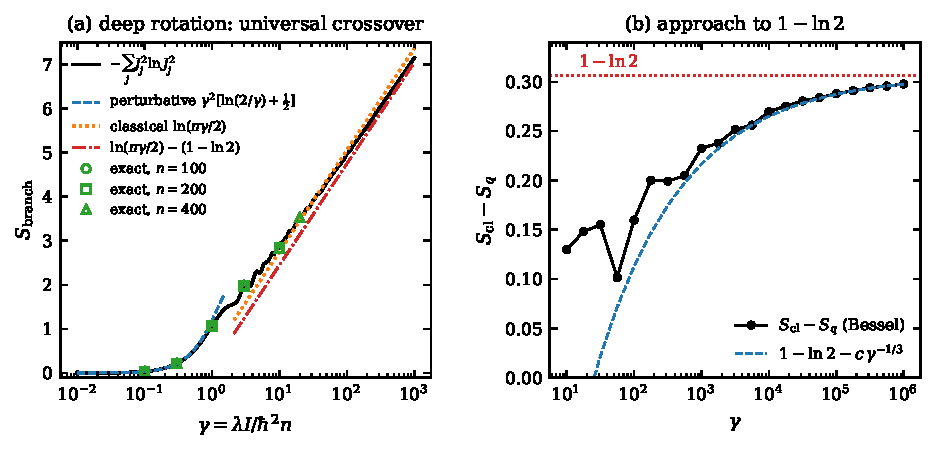
\includegraphics[width=\linewidth]{fig1_rotation.pdf}
\caption{Deep rotation. (a) The branch entropy as a universal function of
$\gamma=\lambda I/\hbar^{2}n$: the Bessel result \eqref{eq:SB} (black), its
small-$\gamma$ (second-order perturbative) limit \eqref{eq:Ssmall} (blue
dashed), the classical arcsine entropy (orange dotted) and the classical entropy
minus $1-\ln2$ (red dash-dotted). Open symbols: exact diagonalisation at
$n=100,200,400$. (b) The deficit $\Scl^{\rm bin}-S_{q}$ from the Bessel weights,
approaching $1-\ln2$ as $\gamma^{-1/3}$.}
\label{fig:rotation}
\end{figure}

\subsection{Interpretation}

In the oscillator problem no conservation law singles out a Schmidt basis: the
reduced density matrix of~\cite{DKS} is doubly degenerate, its eigenvalues
follow the smooth arcsine law, and the two-branch interference is absorbed into
the eigenvectors. For the rotors, conservation of $J$ forces the Schmidt basis
to be the angular-momentum basis (Sec.~\ref{sec:S}), so the interference cannot
be absorbed into the eigenvectors and appears in the eigenvalues, as the
fringes \eqref{eq:fringesgen}. The leading logarithms agree; the constant terms
differ by $1-\ln2$. Equivalently, the classical formula \eqref{eq:Sdiff}
reproduces the quantum entropy if the cell is taken to be $eh/2$ rather than
$h$, since $\ln(e/2)=1-\ln2$. Section~\ref{sec:wigner} locates the same
interference in phase space.

%=============================================================================
\section{Generic energies and the separatrix}
\label{sec:compare}
%=============================================================================

Away from deep rotation we compare \eqref{eq:Smathieu}, computed by exact
diagonalisation in the parity sectors, with \eqref{eq:Sbin}, computed by
adaptive quadrature of \eqref{eq:Wclass} over each cell.
Figure~\ref{fig:separatrix} shows both for $\lambda I/\hbar^{2}=50,200,800$ as
functions of $\Erel/\lambda$.

\begin{figure}[t]
\centering
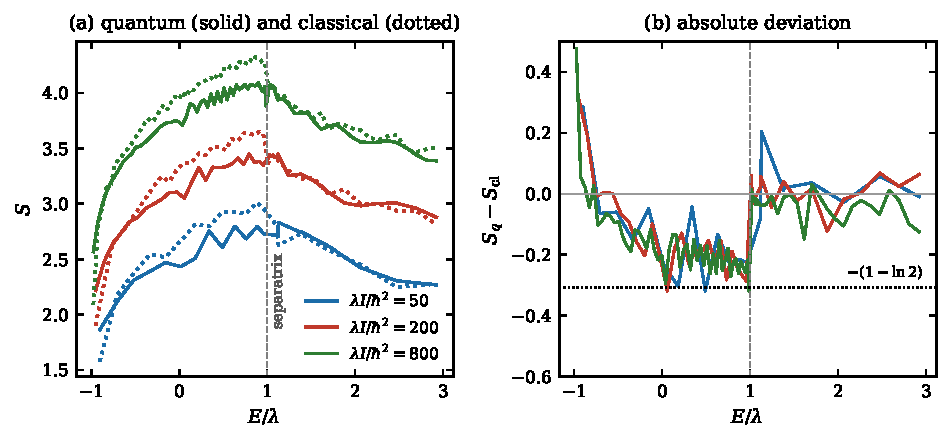
\includegraphics[width=\linewidth]{fig2_separatrix.pdf}
\caption{(a) Quantum entanglement entropy (solid) and classical coarse-grained
entropy (dotted) as functions of $\Erel/\lambda$ for $\lambda I/\hbar^{2}=50$,
$200$ and $800$. The dashed line marks the separatrix. (b) The deviation
$S_{q}-\Scl^{\rm bin}$, with the asymptotic value $-(1-\ln2)$ of
\eqref{eq:main} shown dotted.}
\label{fig:separatrix}
\end{figure}

\emph{Agreement and deficit.} The curves track each other over the whole range.
The quantum entropy lies below the classical one throughout libration, by about
$0.2$, except within a few levels of the bottom of the well, where the band
covers only a handful of cells; above the separatrix it lies below by a smaller
amount that grows with $\lambda$. Relative to $S\approx3$--$4$ this is a few
percent. Figure~\ref{fig:fringes}(a) shows the mechanism: at
$\lambda I/\hbar^{2}=800$, $\Erel/\lambda=1.54$, the quantum weights oscillate
about the classical envelope with full contrast, the total-variation distance
between the two distributions is $0.33$, yet the entropies differ by less than
$1\%$. Figure~\ref{fig:fringes}(b) shows the deficit averaged over the energy
windows $0.2\le\Erel/\lambda\le0.7$ (libration) and $1.5\le\Erel/\lambda\le2.5$
(rotation) as $\lambda I/\hbar^{2}$ grows from $200$ to $51\,200$: in libration it
rises from $0.18$ to $0.24$, in rotation from $0.01$ to $0.15$. Both increase
monotonically towards $1-\ln2$, more slowly than in the pure Wannier--Stark case,
because the bands contain only $10$--$500$ cells and the caustic regions carry a
large share of the weight.

\begin{figure}[t]
\centering
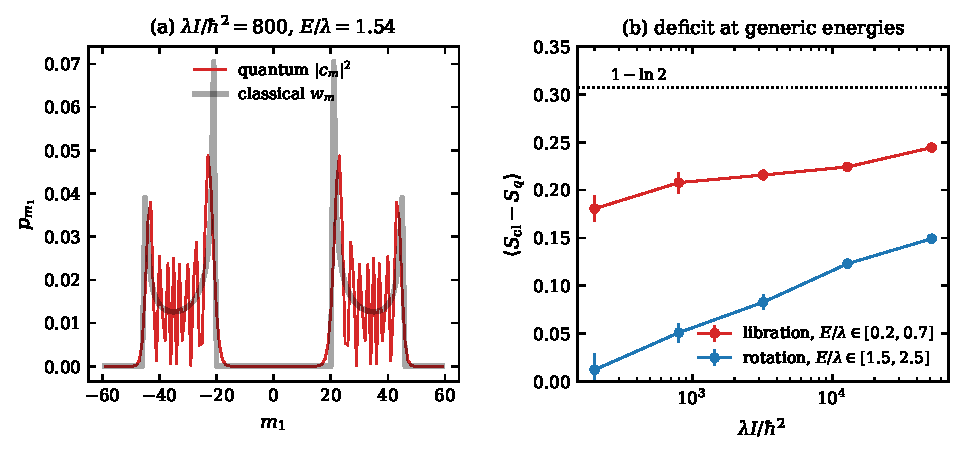
\includegraphics[width=\linewidth]{fig3_fringes.pdf}
\caption{(a) Momentum distribution of rotor 1 at $\lambda I/\hbar^{2}=800$,
$\Erel/\lambda=1.54$: the quantum weights (red) oscillate with full contrast
about the classical cell weights (grey), as \eqref{eq:fringesgen} predicts.
(b) Deficit $\langle\Scl^{\rm bin}-S_{q}\rangle$ averaged over energy windows in
libration and in rotation, against $\lambda$; error bars are standard errors
over the window.}
\label{fig:fringes}
\end{figure}

\emph{The separatrix.} Both entropies are maximal near $\Erel=\lambda$; for
$\lambda I/\hbar^{2}=50$, $200$ and $800$ the quantum maximum is at
$\Erel/\lambda=1.13$, $1.12$ and $0.90$. The classical reason is the cusp of the
support \eqref{eq:support}. On the quantum side this is where the
non-degenerate librational levels give way to the rotational doublets. The
deviation in Fig.~\ref{fig:separatrix}(b) changes abruptly there, because the
fringe structure changes: below the separatrix the two interfering branches are
the two halves of one libration orbit, above it the two halves of one rotation
orbit, and the caustics move from $p=\pm\sqrt{I(\Erel+\lambda)}$ alone to include
$p=\pm\sqrt{I(\Erel-\lambda)}$. The separatrix is the classical locus of an
excited-state quantum phase transition~\cite{CaprioCejnarIachello,Stransky,Cejnar},
and the entropy maximum should be understood in that context.

%=============================================================================
\section{Deep libration}
\label{sec:libration}
%=============================================================================

\subsection{Harmonic approximation}

For $\lambda I/\hbar^{2}\gg1$ the ground state of $h$ is localised near
$\varphi=\pi$. With $x=\varphi-\pi$,
$\lambda\cos\varphi=-\lambda+\tfrac12\lambda x^{2}-\tfrac{1}{24}\lambda x^{4}+\dots$,
\begin{equation}
h=-\lambda+\frac{p^{2}}{2\mu}+\frac12\mu\omega^{2}x^{2}-gx^{4}+\dots,\qquad
\mu=\frac{I}{2},\quad \mu\omega^{2}=\lambda,\quad g=\frac{\lambda}{24},
\label{eq:hho}
\end{equation}
so $\omega=\sqrt{2\lambda/I}$. Neglecting $g$, the ground state is
$u_{0}\propto\exp(-\mu\omega x^{2}/2\hbar)$, with
$\langle p^{2}\rangle=\mu\hbar\omega/2$. Its Fourier coefficients are, up to the
phase $e^{-ik\pi}$, a Gaussian in $k=p/\hbar$ with variance
\begin{equation}
\sigma_{0}^{2}=\frac{\langle p^{2}\rangle}{\hbar^{2}}=\frac{\mu\omega}{2\hbar}
=\frac14\sqrt{\frac{2\lambda I}{\hbar^{2}}} .
\label{eq:sigma0}
\end{equation}

\subsection{Entropy of a sampled Gaussian}

For $p_{k}=e^{-k^{2}/2\sigma^{2}}/Z$ on the integers, Poisson summation gives
\begin{equation}
Z=\sqrt{2\pi}\,\sigma\Big[1+2\sum_{r\ge1}e^{-2\pi^{2}\sigma^{2}r^{2}}\Big],\qquad
\sum_{k}k^{2}p_{k}=\sigma^{2}\left[1+O\big(\sigma^{2}e^{-2\pi^{2}\sigma^{2}}\big)\right].
\end{equation}
Since
$-\ln p_{k}=\ln Z+k^{2}/2\sigma^{2}$,
\begin{equation}
S=\frac12\ln\left(2\pi e\sigma^{2}\right)
+O\!\left(\sigma^{2}e^{-2\pi^{2}\sigma^{2}}\right).
\end{equation}
The discreteness correction is exponentially small. With $\sigma=\sigma_{0}$,
\begin{equation}
S_{0}=\frac12\ln\left(2\pi e\cdot\frac14\sqrt{\frac{2\lambda I}{\hbar^{2}}}\right)
=\frac14\ln\frac{\lambda I}{\hbar^{2}}+\frac12\ln\frac{\pi e}{\sqrt2}.
\end{equation}

\subsection{The leading anharmonic correction}

The quartic term narrows the momentum distribution. The virial theorem,
$\langle[h,xp]\rangle=0$, gives $2\langle T\rangle=\langle xV'\rangle$. With
$V=V_{2}-V_{4}$, $V_{2}=\tfrac12\mu\omega^{2}x^{2}$, $V_{4}=gx^{4}$, one has
$xV'=2V_{2}-4V_{4}$, so $\langle V_{2}\rangle=\langle T\rangle+2\langle V_{4}\rangle$
and $E=\langle T\rangle+\langle V_{2}\rangle-\langle V_{4}\rangle$ gives
$\langle T\rangle=\tfrac12(E-\langle V_{4}\rangle)$. To first order in $g$,
$E=\tfrac12\hbar\omega-g\langle x^{4}\rangle_{0}$ and
$\langle V_{4}\rangle=g\langle x^{4}\rangle_{0}$, with
$\langle x^{4}\rangle_{0}=3\hbar^{2}/4\mu^{2}\omega^{2}$. Therefore
\begin{equation}
\langle p^{2}\rangle=2\mu\langle T\rangle=\frac{\mu\hbar\omega}{2}
-\frac{3g\hbar^{2}}{2\mu\omega^{2}}=\frac{\mu\hbar\omega}{2}-\frac{\hbar^{2}}{16},
\qquad
\sigma^{2}=\sigma_{0}^{2}-\frac{1}{16}.
\end{equation}
The quartic term also makes the distribution non-Gaussian, but this does not
change the entropy at first order: if $p=\phi_{\sigma}(1+\epsilon\eta)$ with
$\phi_{\sigma}$ the Gaussian of the exact variance, then $\eta$ is orthogonal
(with weight $\phi_{\sigma}$) to $1$, $k$ and $k^{2}$, and
$-\sum p\ln p=S[\phi_{\sigma}]-\epsilon\sum\phi_{\sigma}\eta(1+\ln\phi_{\sigma})
+O(\epsilon^{2})=S[\phi_{\sigma}]+O(\epsilon^{2})$, because
$\ln\phi_{\sigma}$ is a quadratic polynomial in $k$. Expanding
$\tfrac12\ln(\sigma_{0}^{2}-\tfrac1{16})$,
\begin{equation}
\boxed{\;
S_{0}=\frac14\ln\frac{\lambda I}{\hbar^{2}}+\frac12\ln\frac{\pi e}{\sqrt2}
-\frac{1}{8\sqrt{2\lambda I/\hbar^{2}}}+O\!\left(\frac{\hbar^{2}}{\lambda I}\right)\;}
\label{eq:S0}
\end{equation}
with $\tfrac12\ln(\pi e/\sqrt2)=0.89908$. For $\lambda I/\hbar^{2}=10$, $40$,
$160$, $640$, $2560$ and $10240$ the residual after the harmonic terms is
$-0.03027$, $-0.01451$, $-0.00712$, $-0.00353$, $-0.00176$ and $-0.00088$, and its
ratio to the predicted correction is $1.083$, $1.039$, $1.019$, $1.009$, $1.005$
and $1.002$ (Fig.~\ref{fig:libration}).

\begin{figure}[t]
\centering
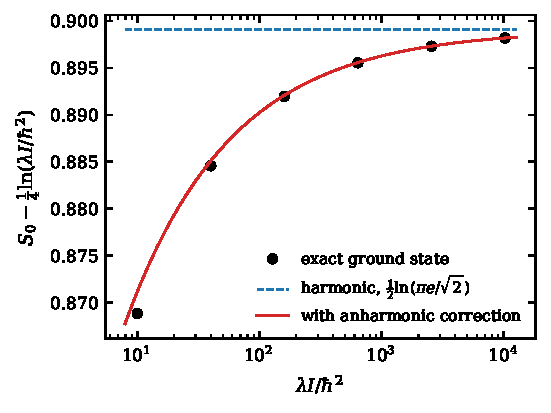
\includegraphics[width=0.55\linewidth]{fig4_libration.pdf}
\caption{Deep libration: $S_{0}-\tfrac14\ln(\lambda I/\hbar^{2})$ for the
ground state from exact diagonalisation (points), the harmonic constant
$\tfrac12\ln(\pi e/\sqrt2)$ (dashed), and \eqref{eq:S0} with the anharmonic
correction (solid).}
\label{fig:libration}
\end{figure}

%=============================================================================
\section{Wigner and Husimi distributions}
\label{sec:wigner}
%=============================================================================

We now ask what happens if the classical microcanonical distribution
\eqref{eq:Wjoint} is replaced by a quantum phase-space distribution of the
eigenstate itself. Throughout this section $\ell$ denotes momentum in units of
$\hbar$.

\subsection{The Wigner function on a circle}

For a single rotor with density matrix $\rho$ and $\braket{\theta}{m}=
e^{im\theta}/\sqrt{2\pi}$, the Wigner function
is~\cite{Mukunda,Bizarro,Rigas}
\begin{equation}
W_{\rho}(\theta,\ell)=\frac{1}{4\pi}\int_{-2\pi}^{2\pi}\dd\xi\;e^{-i\ell\xi}\,
\bra{\theta+\tfrac{\xi}{2}}\rho\ket{\theta-\tfrac{\xi}{2}},\qquad
\ell\in\tfrac12\mathbb{Z}.
\label{eq:Wdef}
\end{equation}
The kernel is $4\pi$-periodic in $\xi$ (a shift of $\xi$ by $4\pi$ moves
$\theta\pm\xi/2$ by $\pm2\pi$), so its Fourier variable $\ell$ runs over the
half-integers. Inserting the basis,
\begin{equation}
\bra{\theta+\tfrac{\xi}{2}}\rho\ket{\theta-\tfrac{\xi}{2}}=\frac{1}{2\pi}
\sum_{m,m'}\rho_{mm'}\,e^{i(m-m')\theta}\,e^{i(m+m')\xi/2},
\end{equation}
and since $\int_{-2\pi}^{2\pi}e^{is\xi}\dd\xi=4\pi\delta_{s0}$ for
$s\in\tfrac12\mathbb{Z}$,
\begin{equation}
W_{\rho}(\theta,\ell)=\frac{1}{2\pi}\sum_{m+m'=2\ell}\rho_{mm'}\,e^{i(m-m')\theta}.
\label{eq:Wmm}
\end{equation}
From \eqref{eq:Wmm}: (i) $W_{\rho}$ is real for Hermitian $\rho$;
(ii) $\sum_{\ell\in\frac12\mathbb{Z}}W_{\rho}(\theta,\ell)=\bra\theta\rho\ket\theta$;
(iii) $\int_{0}^{2\pi}\dd\theta\,W_{\rho}(\theta,\ell)=\rho_{\ell\ell}$ for
$\ell\in\mathbb{Z}$ and $0$ for $\ell\in\mathbb{Z}+\tfrac12$;
(iv) $\Tr(\rho\sigma)=2\pi\sum_{\ell}\int\dd\theta\,W_{\rho}W_{\sigma}$, since
the $\theta$ integral forces $m-m'=n'-n$, which with $m+m'=n+n'$ gives $m=n'$,
$m'=n$. The half-integer rows have zero momentum marginal: they carry only
coherences.

For two rotors the same construction in each variable gives
\begin{equation}
W(\theta_{1},\ell_{1};\theta_{2},\ell_{2})=\frac{1}{(2\pi)^{2}}
\sum_{\substack{m_{1}+m_{1}'=2\ell_{1}\\ m_{2}+m_{2}'=2\ell_{2}}}
\rho_{m_{1}m_{2};m_{1}'m_{2}'}\,
e^{i(m_{1}-m_{1}')\theta_{1}+i(m_{2}-m_{2}')\theta_{2}} .
\label{eq:W2}
\end{equation}
Integrating over $\theta_{2}$ sets $m_{2}'=m_{2}$, after which the sum over
$\ell_{2}$ sums over $m_{2}$ once:
\begin{equation}
\sum_{\ell_{2}\in\frac12\mathbb{Z}}\int_{0}^{2\pi}\dd\theta_{2}\;
W(\theta_{1},\ell_{1};\theta_{2},\ell_{2})
=\frac{1}{2\pi}\sum_{m_{1}+m_{1}'=2\ell_{1}}(\rho_{1})_{m_{1}m_{1}'}
e^{i(m_{1}-m_{1}')\theta_{1}}=W_{\rho_{1}}(\theta_{1},\ell_{1}).
\label{eq:Wmarg}
\end{equation}
\emph{Integrating the Wigner function over the second rotor is the partial
trace.}

\subsection{Eigenstates: the Wigner analogue of the DKS construction}

For an eigenstate $\ket\Psi=\sum_{k}c_{k}\ket{\tfrac M2+k,\tfrac M2-k}$ the
matrix elements are $\rho_{m_{1}m_{2};m_{1}'m_{2}'}=c_{k}\bar c_{k'}$ with
$m_{1}=\tfrac M2+k$, $m_{2}=\tfrac M2-k$, and similarly for the primes. The
constraints in \eqref{eq:W2} become $2\ell_{1}=M+k+k'$, $2\ell_{2}=M-k-k'$, and
the phase is $(k-k')(\theta_{1}-\theta_{2})$. Hence
\begin{equation}
W(\theta_{1},\ell_{1};\theta_{2},\ell_{2})=\frac{1}{2\pi}\,
\delta_{\ell_{1}+\ell_{2},M}\;W_{\rm rel}\!\left(\theta_{1}-\theta_{2},\,
\ell_{1}-\tfrac M2\right),\qquad
W_{\rm rel}(\varphi,\ell)=\frac{1}{2\pi}\sum_{k+k'=2\ell}c_{k}\bar c_{k'}\,
e^{i(k-k')\varphi},
\label{eq:Wfactor}
\end{equation}
where $W_{\rm rel}$ is the Wigner function \eqref{eq:Wmm} of the relative wave
function $u(\varphi)$. The classical distribution \eqref{eq:Wjoint} has the same
skeleton: in the variables \eqref{eq:cmrel},
\begin{equation}
W_{\rm cl}=\frac{1}{2\pi}\,\delta\!\left(J-p_{1}-p_{2}\right)\,
\frac{\delta\!\left(\Erel-H_{\rm rel}(\varphi,p)\right)}{4B},
\label{eq:Wclfactor}
\end{equation}
as follows from $\mathcal{C}=1/8\pi B$ and
$\int\dd\varphi\,\dd p\;\delta(\Erel-H_{\rm rel})=4B$. The factor $1/2\pi$
(uniformity in the centre-of-mass angle) and the conservation of total angular
momentum appear identically; the only difference is the relative factor,
$W_{\rm rel}$ against the microcanonical density on the pendulum level set.

Now carry out the DKS construction with $W$ in place of $W_{\rm cl}$. By
\eqref{eq:Wmarg} and \eqref{eq:Smathieu} the reduced Wigner function is
\begin{equation}
W_{1}(\theta_{1},\ell_{1})=\begin{cases}p_{k}/2\pi, & \ell_{1}=\tfrac M2+k\in
\mathbb{Z}+\tfrac M2,\\[2pt] 0, & \text{otherwise},\end{cases}
\label{eq:W1}
\end{equation}
independent of $\theta_{1}$ and non-negative. Its Boltzmann entropy with the
cell fixed in Sec.~\ref{sec:cell} ($2\pi W_{1}$ is the probability per cell) is
\begin{equation}
-\sum_{\ell_{1}}\int_{0}^{2\pi}\dd\theta_{1}\,W_{1}\ln\left(2\pi W_{1}\right)
=-\sum_{k}p_{k}\ln p_{k}=S_{q}.
\label{eq:SWig}
\end{equation}
\emph{The Wigner version of the classical calculation returns the von Neumann
entropy identically}, for every eigenstate, at every coupling and every
$\hbar$. It contains no semiclassical approximation and no new information.
Two remarks. First, the identity requires $W_{1}\ge0$, which in general fails
for a reduced Wigner function; here it holds because $\rho_{1}$ is diagonal,
i.e.\ because of $J$ conservation. Second, \eqref{eq:SWig} answers the question
posed in the Introduction: replacing the classical distribution by the Wigner
function does not give a ``classical'' entropy, it gives the quantum one. The
informative object is the relation between $W_{\rm rel}$ and the classical
level set, to which we turn.

\subsection{Where the classical distribution sits inside the Wigner function}

Figure~\ref{fig:wigner} shows $W_{\rm rel}$ for a librating and a rotating level
at $\lambda I/\hbar^{2}=200$. Its structure is that described by Berry for
one-dimensional eigenstates~\cite{Berry77,OzorioRep}. The function is large on
the classical curve $H_{\rm rel}=\Erel$ (dashed), with an Airy profile across
it, and it oscillates inside: at a point $(\varphi,\ell)$ there is a
contribution from every chord of the classical curve centred on that point,
with a phase equal to the symplectic area between chord and curve in units of
$\hbar$. The oscillations make $W_{\rm rel}$ strongly negative: the negativity
volume~\cite{Kenfack} $\sum_{\ell}\int\dd\varphi\,|W_{\rm rel}|-1$ is $5.86$ and
$5.43$ for the two states shown. Averaged over a phase-space region large on
the scale $\hbar$ but small classically, the chord terms cancel and
$W_{\rm rel}$ reduces to the microcanonical density on the
curve~\cite{Berry77,Voros}.

\begin{figure}[t]
\centering
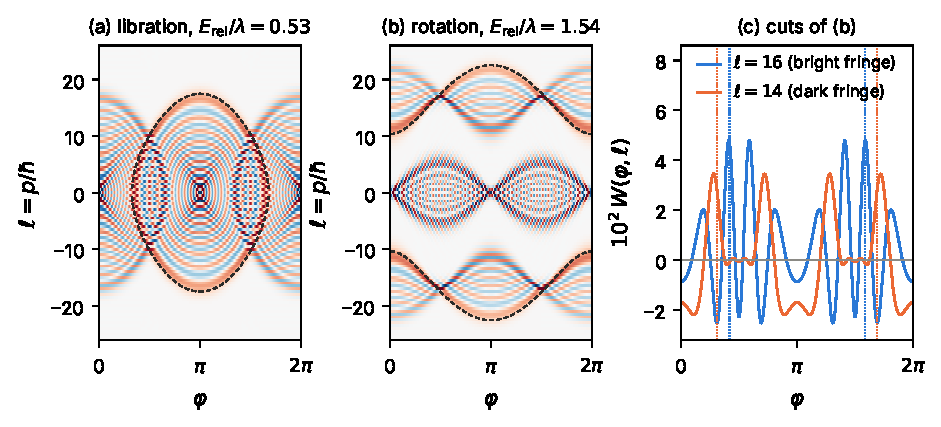
\includegraphics[width=\linewidth]{fig5_wigner.pdf}
\caption{Relative Wigner function $W_{\rm rel}(\varphi,\ell)$, Eq.~\eqref{eq:Wfactor},
at $\lambda I/\hbar^{2}=200$ (red positive, blue negative; both integer and
half-integer rows are shown). (a) Librating level, $\Erel/\lambda=0.53$;
(b) rotating level, $\Erel/\lambda=1.54$ (odd parity: the band near $\ell=0$ is
the interference between the two counter-rotating tori). Dashed: the classical
curve $\ell^{2}+\lambda\cos\varphi=\Erel$. (c) Cuts of (b) at $\ell=16$ (bright
fringe of $p_{\ell}$) and $\ell=14$ (dark fringe); dotted lines mark the
classical angles $\pm\phi_{\ell}$. Away from them the cut oscillates: these are
the chord terms that survive the integration over $\varphi$.}
\label{fig:wigner}
\end{figure}

The two operations ``smooth'' and ``integrate over $\varphi$'' do not commute,
and this is the phase-space content of Sec.~\ref{sec:rotation}. Integrating
$W_{\rm rel}$ over $\varphi$ at fixed integer $\ell$ collects (a) the two
points of the classical curve at momentum $\ell$, $\varphi=\pm\phi_{\ell}$,
which give the classical weight $w_{\ell}$, and (b) the horizontal chord joining
them, which is centred on $\varphi=0$ and on $\varphi=\pi$ and gives
$w_{\ell}\cos\Phi_{\ell}$. Together they produce \eqref{eq:fringesgen}. At
$\ell=14$ in Fig.~\ref{fig:wigner}(c), for example, integrating over windows of
half-width $0.35$ around $\pm\phi_{\ell}$ gives $+0.022$, around $0$ and $\pi$
gives $-0.027$, and the full integral is $p_{14}=7\times10^{-4}$, a dark
fringe. On half-integer rows the chord contributions at $\varphi=0$ and $\pi$
have opposite signs ($\mp0.012$ at $\ell=16.5$) and the marginal vanishes, as
property (iii) requires. Smoothing first removes the chord terms and gives the
classical distribution; integrating first keeps them. \emph{The constant
$1-\ln2$ is the entropy carried by the chord terms of the Wigner function.}

\subsection{The Husimi function and the Wehrl entropy}

The natural way to remove the chord terms in a quantum language is the Husimi
function~\cite{Husimi}, the expectation value in coherent states. On the circle
we use~\cite{KRP,GonzalezOlmo}
\begin{equation}
\ket{\theta,\ell}=\sum_{m\in\mathbb{Z}}\sqrt{g_{\sigma}(m-\ell)}\;e^{-im\theta}
\ket m,\qquad g_{\sigma}(x)=\frac{e^{-x^{2}/2\sigma^{2}}}{\sqrt{2\pi}\,\sigma},
\qquad\theta\in[0,2\pi),\ \ell\in\mathbb{R}.
\label{eq:cs}
\end{equation}
In the angle representation this is a wave packet centred on $\theta$ with
mean momentum $\ell$, momentum width $\sigma$ and angular width $1/2\sigma$. The
resolution of the identity,
$\int_{0}^{2\pi}\frac{\dd\theta}{2\pi}\int_{-\infty}^{\infty}\dd\ell\,
\ketbra{\theta,\ell}{\theta,\ell}=\sum_{m}\ketbra mm\int\dd\ell\,g_{\sigma}(m-\ell)
=\mathbb{1}$, holds exactly; the measure $\dd\theta\,\dd\ell/2\pi$ is the phase
space measure with cell $h$. By Poisson summation the norm is
$\braket{\theta,\ell}{\theta,\ell}=\sum_{m}g_{\sigma}(m-\ell)=1+2\sum_{r\ge1}
e^{-2\pi^{2}\sigma^{2}r^{2}}\cos2\pi r\ell$, within $1.5\%$ of unity for
$\sigma\ge\tfrac12$ and within $10^{-8}$ for $\sigma\ge1$; we restrict to
$\sigma\ge\tfrac12$.

For the reduced state \eqref{eq:Smathieu} the Husimi function
$Q(\theta,\ell)=\bra{\theta,\ell}\rho_{1}\ket{\theta,\ell}$ is independent of
$\theta$,
\begin{equation}
Q(\ell)=\sum_{m}p_{m}\,g_{\sigma}(\ell-m),
\label{eq:Q}
\end{equation}
the Schmidt weights smoothed by a Gaussian of width $\sigma$, and the Wehrl
entropy~\cite{Wehrl,Wehrl79} is
\begin{equation}
\SW(\sigma)=-\int_{0}^{2\pi}\frac{\dd\theta}{2\pi}\int\dd\ell\;Q\ln Q
=-\int\dd\ell\;Q(\ell)\ln Q(\ell).
\label{eq:SW}
\end{equation}
The same operation applied to the classical density gives
$Q_{\rm cl}=w*g_{\sigma}$ and $\SW[w](\sigma)$, which tends to $\Scl$ of
\eqref{eq:Sdiff} as $\sigma\to0$. We write $\SW[p]$ when the distinction
matters.

\emph{Bounds.} Let $s(\ell)=\sum_{m}g_{\sigma}(\ell-m)$. Concavity of
$\eta(x)=-x\ln x$ (Jensen's inequality with weights $g_{\sigma}(\ell-m)/s$) gives
$\eta(Q)\ge\sum_{m}g_{\sigma}(\ell-m)\eta(p_{m})-Q\ln s$, and integrating over
$\ell$,
\begin{equation}
S_{q}-\epsilon_{\sigma}\;\le\;\SW\;\le\;S_{q}+\tfrac12\ln\left(2\pi e\sigma^{2}\right),
\qquad \epsilon_{\sigma}\le2e^{-2\pi^{2}\sigma^{2}}(1+O(e^{-2\pi^{2}\sigma^{2}})).
\label{eq:bounds}
\end{equation}
The lower bound is the Berezin--Lieb (Wehrl) inequality~\cite{Berezin,Wehrl79,Lieb};
the upper bound follows from writing $Q$ as the distribution of $X=M+Z$, with
$M$ distributed as $p_{m}$ and $Z$ an independent Gaussian of width $\sigma$, and
$h(X)\le H(M)+h(Z)$~\cite{CoverThomas}.

\subsection{Deep rotation: the Wehrl entropy in closed form}

In deep rotation the Husimi entropy can be computed from the fringe structure
\eqref{eq:fringes}. Over a stretch of many cells around $j_{0}$, $w$ is nearly
constant and $\Phi_{j}\simeq\Phi_{0}+\kappa(j-j_{0})$ with $\kappa=-2\beta$ by
\eqref{eq:wavenumber}. By Poisson summation,
\begin{equation}
\sum_{j}e^{i\kappa j}g_{\sigma}(x-j)=\sum_{r\in\mathbb{Z}}
e^{i(\kappa+2\pi r)x}\,e^{-\sigma^{2}(\kappa+2\pi r)^{2}/2}.
\end{equation}
For $\sigma\gtrsim1$ only the alias closest to zero survives, and
\begin{equation}
Q(x)\simeq w(x)\left[1+A\cos\tilde\Phi(x)\right],\qquad
A=e^{-\sigma^{2}d(\kappa)^{2}/2},\qquad d(\kappa)=\min_{r}|\kappa+2\pi r|,
\label{eq:Qfringe}
\end{equation}
where $\tilde\Phi$ varies on the scale of a few cells. The smoothing does not
remove the fringes; it reduces their contrast from $1$ to $A$. Inserting
\eqref{eq:Qfringe} into \eqref{eq:SW} and averaging over the fast phase as in
Sec.~\ref{sec:rotation},
\begin{equation}
\SW\simeq\Scl-\int\dd x\;w(x)\,f\big(A(x)\big),
\label{eq:SWfringe}
\end{equation}
with the contrast function
\begin{equation}
f(A)=\big\langle(1+A\cos\Phi)\ln(1+A\cos\Phi)\big\rangle_{\Phi}
=\ln\frac{1+\sqrt{1-A^{2}}}{2}+1-\sqrt{1-A^{2}},
\label{eq:fA}
\end{equation}
derived in \ref{app:integrals}; $f(1)=1-\ln2$ recovers \eqref{eq:main}. With
$j=\gamma\cos\beta$ the arcsine weight is uniform in $\beta$, and
$d(-2\beta)=\min(2\beta,2\pi-2\beta)$. Subtracting \eqref{eq:main},
\begin{equation}
\boxed{\;\SW(\sigma)-S_{q}=\left(1-\ln2\right)-D(\sigma),\qquad
D(\sigma)=\frac{2}{\pi}\int_{0}^{\pi/2}f\!\left(e^{-2\sigma^{2}\beta^{2}}\right)
\dd\beta\;}
\label{eq:Dsigma}
\end{equation}
\emph{Uniformity in $\gamma$.} The approximations \eqref{eq:fringesgen} and
\eqref{eq:Qfringe} both fail near the band edges, which is why $\Scl-S_{q}$
approaches $1-\ln2$ only as $\gamma^{-1/3}$. But there $\beta\to0$ or $\pi$, so
$A\to1$: the edge fringes are slow and are not touched by the smoothing. The
integrand of $\SW-S_{q}$, $f(1)-f(A)$, vanishes where the approximations fail,
and \eqref{eq:Dsigma} holds without the $\gamma^{-1/3}$ correction.

\emph{Large $\sigma$.} For $\sigma\gg1$ the integrand is non-negligible only for
$\beta\lesssim1/\sigma$, the upper limit can be sent to infinity, and the series
$f(A)=\sum_{n\ge1}\binom{2n}{n}A^{2n}/[4^{n}2n(2n-1)]$ (\ref{app:integrals})
integrates term by term:
\begin{equation}
D(\sigma)\simeq\frac{c_{1}}{\sigma},\qquad
c_{1}=\frac{1}{2\sqrt\pi}\sum_{n\ge1}\frac{\binom{2n}{n}}{4^{n}\,2n(2n-1)\sqrt n}
=0.080171\ldots
\label{eq:c1}
\end{equation}
The first term alone gives $1/8\sqrt\pi=0.0705$; for $\sigma\ge1$ the asymptotic
form is accurate to better than $10^{-5}$.

\emph{Numerical test.} Table~\ref{tab:husimi_rot} compares \eqref{eq:Dsigma} with
the Wehrl entropy of the Bessel weights. At $\gamma=10^{4}$ the agreement is
within $0.001$ for $1\le\sigma\le4$ (within $0.005$ at $\gamma=10^{3}$), and
$\SW-S_{q}$ is the same at $\gamma=10^{3}$ and $10^{4}$ to within $0.004$,
although $\Scl-S_{q}$ changes from $0.212$ to $0.263$ between them. At $\sigma=\tfrac12$ the second alias, which
matters near $\beta=\pi/2$ (fringes of period two cells), lowers the result by
$0.003$. At $\gamma=30$ and $100$ the larger widths begin to resolve the band
itself and the Wehrl entropy rises above \eqref{eq:Dsigma}.
Figure~\ref{fig:husimi}(a) shows the $\sigma$ dependence. The equal-smoothing
gap in the sixth column decomposes as
$\SW[w]-\SW[p]=D(\sigma)-[(1-\ln2)-(\Scl-S_{q})]+[\SW[w]-\Scl]$: the residual
fringe loss, minus the caustic correction to the unsmoothed deficit, plus the
broadening of the classical band edges. At $\gamma=10^{4}$ the three terms
reproduce the column to $0.004$.

\begin{table}[t]
\centering
\caption{Wehrl entropy of the deep-rotation Schmidt weights $p_{j}=J_{j}^{2}(\gamma)$
against Eq.~\eqref{eq:Dsigma}. $\SW[w]$ is the Wehrl entropy of the arcsine law
smoothed with the same $\sigma$. $\Scl=\ln(\pi\gamma/2)$.}
\label{tab:husimi_rot}
\small
\renewcommand{\arraystretch}{1.12}
\begin{tabular}{rr cccc c}
\toprule
$\gamma$ & $\sigma$ & $\SW[p]-S_{q}$ & $(1-\ln2)-D(\sigma)$ & $\SW[p]-\Scl$ &
$\SW[w]-\SW[p]$ & $\Scl-S_{q}$\\
\midrule
$10^{2}$ & $0.5$ & 0.1406 & 0.1502 & 0.0453 & 0.0364 & \multirow{4}{*}{0.0953}\\
         & $1$   & 0.2218 & 0.2267 & 0.1265 & $-0.0110$ & \\
         & $2$   & 0.2713 & 0.2668 & 0.1760 & $-0.0127$ & \\
         & $4$   & 0.3300 & 0.2868 & 0.2347 & $-0.0040$ & \\
\midrule
$10^{3}$ & $0.5$ & 0.1468 & 0.1502 & $-0.0654$ & 0.0912 & \multirow{4}{*}{0.2122}\\
         & $1$   & 0.2274 & 0.2267 & 0.0152 & 0.0213 & \\
         & $2$   & 0.2680 & 0.2668 & 0.0558 & $-0.0041$ & \\
         & $4$   & 0.2916 & 0.2868 & 0.0795 & $-0.0064$ & \\
\midrule
$10^{4}$ & $0.5$ & 0.1468 & 0.1502 & $-0.1165$ & 0.1247 & \multirow{4}{*}{0.2633}\\
         & $1$   & 0.2274 & 0.2267 & $-0.0359$ & 0.0475 & \\
         & $2$   & 0.2675 & 0.2668 & 0.0042 & 0.0121 & \\
         & $4$   & 0.2877 & 0.2868 & 0.0244 & $-0.0013$ & \\
\bottomrule
\end{tabular}
\end{table}

Three consequences follow. First, the Husimi entropy of the quantum state does
\emph{not} converge to the classical entropy at fixed $\sigma$: as
$\gamma\to\infty$,
\begin{equation}
\SW(\sigma)-\Scl\;\longrightarrow\;-D(\sigma)\simeq-\frac{0.080}{\sigma},
\label{eq:SWScl}
\end{equation}
because a coherent state of fixed width only reduces the contrast of the fine
fringes and does not remove it. Second, the classical value is reached only in
the double limit $1\ll\sigma\ll\gamma$, the upper bound being needed so that
the smoothing does not broaden the band itself. Third, the remaining gap closes
algebraically, as $1/\sigma$, not exponentially: fringes of all wavenumbers
down to zero are present near the band edges, and a Gaussian of any width
leaves the slowest of them intact.

\subsection{Generic energies}

At generic energies the local fringe wavenumber is $2\phi_{k}$, with $\phi_{k}$
the classical relative angle at momentum $k$ (Sec.~\ref{sec:rotation}), and the
same argument gives $\SW-S_{q}\simeq(1-\ln2)-D(\sigma;\Erel)$ with
\begin{equation}
D(\sigma;\Erel)=\Big\langle f\!\left(e^{-\sigma^{2}d(2\phi)^{2}/2}\right)
\Big\rangle_{\rm orbit},
\label{eq:Dgen}
\end{equation}
the average being over one period of the classical relative motion (the
measure $w\,\dd p$). Table~\ref{tab:husimi_gen} gives window averages at
$\lambda I/\hbar^{2}=200$ and $800$, computed with the classical density sampled
uniformly in time along the orbit, which avoids the band-edge singularities.
For $\sigma\le1$, $\SW[p]-S_{q}$ agrees with \eqref{eq:Dgen} to within
$0.03$; for $\sigma=2$ the bands, only $10$--$40$ cells wide, are themselves
broadened and the Wehrl entropy is larger than \eqref{eq:Dgen} predicts.

\begin{table}[t]
\centering
\caption{Window averages over $0.2\le\Erel/\lambda\le0.7$ (libration) and
$1.5\le\Erel/\lambda\le2.5$ (rotation), all levels of the sector $M=0$.
Column 3 is the unsmoothed comparison of Sec.~\ref{sec:compare}.}
\label{tab:husimi_gen}
\footnotesize
\setlength{\tabcolsep}{4pt}
\renewcommand{\arraystretch}{1.12}
\begin{tabular}{llc c cccc}
\toprule
$\frac{\lambda I}{\hbar^{2}}$ & regime & $\Scl^{\rm bin}-S_{q}$ & $\sigma$ &
$\SW[p]-S_{q}$ & $(1-\ln2)-D(\sigma;\Erel)$ & $\SW[w]-\SW[p]$ & $\SW[w]-\Scl$\\
\midrule
200 & libration & 0.180 & 0.5 & 0.193 & 0.204 & $\phantom{-}0.025$ & 0.147\\
    &           &       & 1   & 0.284 & 0.270 & $-0.007$ & 0.207\\
    &           &       & 2   & 0.364 & 0.289 & $-0.002$ & 0.292\\
\midrule
200 & rotation  & 0.012 & 0.5 & 0.146 & 0.146 & $-0.046$ & 0.361\\
    &           &       & 1   & 0.273 & 0.223 & $-0.026$ & 0.508\\
    &           &       & 2   & 0.459 & 0.264 & $-0.007$ & 0.713\\
\midrule
800 & libration & 0.208 & 0.5 & 0.202 & 0.204 & $\phantom{-}0.031$ & 0.104\\
    &           &       & 1   & 0.284 & 0.270 & $-0.008$ & 0.147\\
    &           &       & 2   & 0.339 & 0.289 & $-0.003$ & 0.207\\
\midrule
800 & rotation  & 0.051 & 0.5 & 0.144 & 0.146 & $-0.030$ & 0.256\\
    &           &       & 1   & 0.246 & 0.223 & $-0.027$ & 0.361\\
    &           &       & 2   & 0.374 & 0.264 & $-0.009$ & 0.508\\
\bottomrule
\end{tabular}
\end{table}

The equal-smoothing comparison is the fair one: quantum and classical
distributions seen through the same coherent state. Its outcome is shown in
Fig.~\ref{fig:husimi}(b) level by level at $\lambda I/\hbar^{2}=800$. For
$\sigma=1$ the two Wehrl entropies agree to within $0.04$, and for $\sigma=2$ to
within $0.015$, at every level with $-0.5<\Erel/\lambda<0.8$ or
$1.2<\Erel/\lambda<3$, at both couplings; the window averages in
Table~\ref{tab:husimi_gen} are below $0.03$ and $0.01$. The gap grows only close
to the separatrix, where the classical period diverges. The unsmoothed deficit,
by contrast, is about $0.2$ in libration. The agreement is achieved, however, by moving \emph{both} entropies:
the last column of Table~\ref{tab:husimi_gen} shows that $\SW[w]$ exceeds the
classical entropy $\Scl$ by $0.1$--$0.7$, depending on $\sigma$ and on the
width of the band.

\begin{figure}[t]
\centering
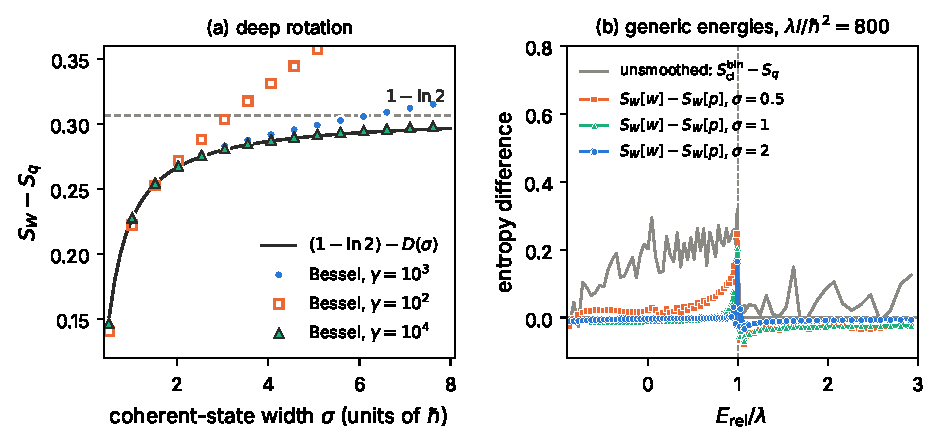
\includegraphics[width=\linewidth]{fig6_husimi.pdf}
\caption{(a) Deep rotation: excess of the Wehrl entropy over the von Neumann
entropy as a function of the coherent-state width, Eq.~\eqref{eq:Dsigma}
(solid), against the Bessel weights at $\gamma=10^{2},10^{3},10^{4}$ (symbols).
At fixed $\sigma$ the excess is independent of $\gamma$ once $\sigma\ll\gamma$;
the full deficit $1-\ln2$ (dashed) is recovered only as $\sigma\to\infty$.
(b) Generic energies at $\lambda I/\hbar^{2}=800$: difference between the Wehrl
entropies of the classical and the quantum momentum distributions for
$\sigma=0.5,1,2$, and the unsmoothed difference $\Scl^{\rm bin}-S_{q}$ (grey).
The dashed line marks the separatrix.}
\label{fig:husimi}
\end{figure}

\subsection{What the phase-space route achieves}

The three distributions --- classical, Wigner, Husimi --- give three different
answers, and the rotor pair makes the relation between them exact.
\begin{enumerate}
\item The \emph{Wigner} function of the reduced state is the marginal of the
two-rotor Wigner function, and its entropy is the von Neumann entropy,
identically \eqref{eq:SWig}. Using it in place of the classical distribution
reproduces the quantum answer, including the deficit $1-\ln2$.
\item The \emph{classical} distribution is the Wigner function with its chord
terms averaged away \emph{before} marginalisation. The constant $1-\ln2$ is the
entropy of the chord terms, which survive the marginalisation as full-contrast
fringes because conservation of $J$ fixes the Schmidt basis.
\item The \emph{Husimi} function removes the chord terms only partially. Its
entropy exceeds $S_{q}$ by $(1-\ln2)-D(\sigma)$, with $D$ in closed form, and
quantum and classical Husimi entropies agree to $O(D(\sigma))$, i.e.\ to
$\simeq0.08/\sigma$ in deep rotation and, at generic energies away from the
separatrix, to $0.04$ for $\sigma=1$ and $0.015$ for $\sigma=2$. But each Husimi entropy depends on $\sigma$, and no value of
$\sigma$ is singled out by the problem. The coherent-state width therefore takes
over the role of the cell $\Delta$ in the oscillator problem of~\cite{DKS}: a
parameter not fixed by the classical theory, whose choice decides the constant
term. The cell itself, by contrast, remains fixed at $h$ by the resolution of
the identity.
\end{enumerate}
One choice of $\sigma$ suggests itself: the momentum width $\sigma_{0}\propto
(\lambda I/\hbar^{2})^{1/4}$ of the pendulum's own ground state,
Eq.~\eqref{eq:sigma0}, the analogue of the coherent states of an oscillator.
With it the residual gap $D(\sigma_{0})\propto(\lambda I/\hbar^{2})^{-1/4}$
vanishes in the semiclassical limit, but only slowly, and the choice is a
convention rather than a consequence of the dynamics.

%=============================================================================
\section{Discussion}
\label{sec:disc}
%=============================================================================

We have carried the programme of~\cite{DKS} from coupled oscillators to coupled
rotors in the semiclassical regime, and extended it from the classical
microcanonical distribution to the Wigner and Husimi distributions of the
eigenstate.

\emph{The cell is fixed, and the equality is not exact.} Compactness quantises
the angular momentum, so the classical distribution is coarse-grained onto the
integers that label the Schmidt weights and the comparison contains no free
constant. With nothing to adjust, the quantum entropy lies below the classical
one by $1-\ln2$ in the semiclassical limit. We derived this in deep rotation,
where the Schmidt weights are $J_{j}^{2}(\gamma)$ and the classical weights the
arcsine law, and confirmed it to $\gamma=10^{6}$; at generic energies the same
deficit is approached more slowly. The leading logarithms agree, as for the
oscillators.

\emph{Why oscillators and rotors differ.} The constant comes from the
interference of the two classical branches compatible with one value of the
observed momentum. For the rotors conservation of total angular momentum fixes
the Schmidt basis, so the interference appears in the Schmidt weights; for the
oscillators it is absorbed into the eigenvectors. In phase space, the
interference is the chord structure of the Wigner function, which marginalises
into the Schmidt weights intact.

\emph{Phase-space distributions.} Replacing the classical distribution by the
Wigner function gives back the von Neumann entropy, identically; replacing it by
the Husimi function gives an entropy between the quantum and classical ones,
with a closed-form dependence on the coherent-state width. The Husimi route
makes the quantum and classical distributions agree to $O(1/\sigma)$ when both
are smoothed equally, but it does so by introducing a width that the problem
does not fix. In this sense the rotor pair sharpens the conclusion of~\cite{DKS}:
there is no classical calculation that reproduces the entanglement entropy
including its constant term without one conventional parameter, be it a cell
(oscillators), a coherent-state width (Husimi), or --- when both are fixed, as
here --- an explicit correction $1-\ln2$.

\emph{The separatrix and deep libration.} Both entropies are maximal near the
separatrix, where the support of the classical momentum distribution has a cusp
and where the excited-state quantum phase transition of the pendulum is
located~\cite{CaprioCejnarIachello,Stransky,Cejnar}. In deep libration the
ground-state entropy is $\tfrac14\ln(\lambda I/\hbar^{2})+\tfrac12\ln(\pi e/\sqrt2)$
up to an anharmonic correction $-[8\sqrt{2\lambda I/\hbar^{2}}]^{-1}$, which we
have verified to three digits.

\emph{Outlook.} Coupling $N>2$ rotors makes the relative motion non-integrable;
whether the constant $1-\ln2$ and the Husimi law \eqref{eq:Dsigma} survive chaos
is the question most relevant to the high-energy setting that
motivated~\cite{DKS}. The Wigner and Husimi functions are also natural tools
for the dynamics of entanglement after a quench of $\lambda$ across the
separatrix, which the Mathieu machinery of Sec.~\ref{sec:model} makes
tractable.

\begin{center}\rule{0.4\linewidth}{0.4pt}\end{center}

\appendix

%=============================================================================
\section{Integrals}
\label{app:integrals}
%=============================================================================

\paragraph{A.1. A logarithmic integral} Let
$I_{s}=\int_{0}^{\pi}\ln\sin u\,\dd u=2\int_{0}^{\pi/2}\ln\sin u\,\dd u
=2\int_{0}^{\pi/2}\ln\cos u\,\dd u$. Adding the last two forms,
\begin{equation}
2I_{s}=2\int_{0}^{\pi/2}\ln\frac{\sin2u}{2}\,\dd u
=\int_{0}^{\pi}\ln\sin v\,\dd v-\pi\ln2=I_{s}-\pi\ln2,
\end{equation}
so $I_{s}=-\pi\ln2$; equivalently $\int_{0}^{\pi}\ln|\cos t|\,\dd t=-\pi\ln2$.

\paragraph{A.2. Entropy of the arcsine law} For $w(j)=1/(\pi\sqrt{\gamma^{2}-j^{2}})$
put $j=\gamma\cos\beta$; then $w\,\dd j=\dd\beta/\pi$ and
\begin{equation}
-\int w\ln w\,\dd j=\ln\pi+\frac{1}{\pi}\int_{0}^{\pi}\ln\left(\gamma\sin\beta\right)
\dd\beta=\ln\frac{\pi\gamma}{2}.
\end{equation}

\paragraph{A.3. The phase average} With $1+\cos\Phi=2\cos^{2}(\Phi/2)$ and A.1,
$\frac{1}{2\pi}\int_{0}^{2\pi}\ln(1+\cos\Phi)\dd\Phi=\ln2-2\ln2=-\ln2$.
Integrating by parts,
$\frac{1}{2\pi}\int_{0}^{2\pi}\cos\Phi\ln(1+\cos\Phi)\dd\Phi
=\frac{1}{2\pi}\int_{0}^{2\pi}\frac{\sin^{2}\Phi}{1+\cos\Phi}\dd\Phi
=\frac{1}{2\pi}\int_{0}^{2\pi}(1-\cos\Phi)\dd\Phi=1$. The sum is $1-\ln2$.

\paragraph{A.4. Band integrals} \emph{Rotation:} with $u=\pi-2t$,
$\Erel-\lambda\cos u=(\Erel+\lambda)(1-k^{2}\sin^{2}t)$,
$k^{2}=2\lambda/(\Erel+\lambda)$, and $B=\tfrac{\sqrt I}{2}\cdot
\tfrac{2}{\sqrt{\Erel+\lambda}}\int_{0}^{\pi/2}\dd t\,(1-k^{2}\sin^{2}t)^{-1/2}$.
\emph{Libration:} $u\in[u_{0},\pi]$ with $\cos u_{0}=\Erel/\lambda$; with
$v=\pi-u$ and $\sin(v/2)=\kappa\sin t$, $\kappa^{2}=(\Erel+\lambda)/2\lambda$,
one has $\Erel+\lambda\cos v=(\Erel+\lambda)\cos^{2}t$ and
$\dd v=2\kappa\cos t\,\dd t/\sqrt{1-\kappa^{2}\sin^{2}t}$, so
$B=\sqrt{I/2\lambda}\,\mathsf{K}(\kappa)$. The same substitutions parametrise
the orbit uniformly in time, $\dd t_{\rm orbit}\propto\dd t/\sqrt{1-k^{2}\sin^{2}t}$,
which we use to sample the classical density in Sec.~\ref{sec:wigner}. Near the
separatrix $\mathsf{K}(k)=\ln(4/k')+O(k'^{2}\ln k')$, $k'=\sqrt{1-k^{2}}$.

\paragraph{A.5. The contrast function $f(A)$} Let
$F(A)=\langle\ln(1+A\cos\Phi)\rangle_{\Phi}$ and
$G(A)=\langle\cos\Phi\ln(1+A\cos\Phi)\rangle_{\Phi}$ for $0\le A\le1$, and
$s=\sqrt{1-A^{2}}$. The standard result~\cite{GR}
$F(A)=\ln[(1+s)/2]$ generalises A.3. Integrating by parts as in A.3,
$G=A\langle\sin^{2}\Phi/(1+A\cos\Phi)\rangle$. With $u=1+A\cos\Phi$,
$\sin^{2}\Phi=(A^{2}-1+2u-u^{2})/A^{2}$, and using $\langle u^{-1}\rangle=1/s$ and
$\langle u\rangle=1$,
\begin{equation}
G=\frac{1}{A}\left[(A^{2}-1)\frac{1}{s}+2-1\right]=\frac{1-s}{A},\qquad
f(A)=F+AG=\ln\frac{1+s}{2}+1-s .
\end{equation}
Alternatively, expanding $(1+y)\ln(1+y)=y+\sum_{k\ge2}(-1)^{k}y^{k}/k(k-1)$ with
$y=A\cos\Phi$ and $\langle\cos^{2n}\Phi\rangle=\binom{2n}{n}4^{-n}$,
\begin{equation}
f(A)=\sum_{n\ge1}\frac{\binom{2n}{n}}{4^{n}\,2n(2n-1)}\,A^{2n}
=\frac{A^{2}}{4}+\frac{A^{4}}{32}+\frac{A^{6}}{96}+\dots
\end{equation}
With $\int_{0}^{\infty}e^{-4n\sigma^{2}\beta^{2}}\dd\beta=\sqrt\pi/(4\sigma\sqrt n)$
this gives \eqref{eq:c1}.

%=============================================================================
\section{Numerical methods and verification}
\label{app:num}
%=============================================================================

All numerics use $\hbar=I=1$ and the sector $M=0$. The pendulum Hamiltonian is
diagonalised in the two parity sectors (Sec.~\ref{sec:parity}) with truncation
$|k|\le N=8\sqrt{\lambda}+150$, the weight on the boundary states being below
$10^{-6}$. Classical cell weights \eqref{eq:Sbin} are computed by adaptive
quadrature with the band-edge singularities supplied to the routine; for the
arcsine law they are evaluated in closed form. Bessel weights are summed over
$|j|\le\gamma+40\gamma^{1/3}+50$. The Wigner function is evaluated from
\eqref{eq:Wfactor} on $720$ angles. Wehrl entropies of discrete weights are
computed exactly on a sub-lattice of $K\ge10/\sigma$ points per cell by
convolution; Wehrl and differential entropies of the classical density are
computed by sampling the orbit uniformly in time (A.4) with $2\times10^{5}$
points, histogramming at resolution $0.01$ and convolving. Table~\ref{tab:checks}
collects the comparisons quoted in the text.

\begin{table}[h]
\centering
\caption{Analytic results against exact numerics ($\hbar=I=1$). Mathieu checks
at $q=14.6$.}
\label{tab:checks}
\small
\renewcommand{\arraystretch}{1.12}
\begin{tabular}{lll}
\toprule
quantity & analytic & numerical\\
\midrule
$M=0$ lowest level vs $a_{0}(q)/4$ & $-5.4542890$ & $-5.4542890$ \\
$M=0$ third level vs $a_{2}(q)/4$ & 1.3368673 & 1.3368673 \\
$M=1$ lowest level vs $b_{1}(q)/4$ & $-5.4542787$ & $-5.4542787$ \\
$M=1$ second level vs $a_{1}(q)/4$ & $-1.9036729$ & $-1.9036729$ \\
$N_{\rm lib}$ at $\lambda I/\hbar^{2}=800$ vs $(4/\pi)\sqrt q$ & 50.92958 & 51 \\
$B$, $\Erel=300$, $\lambda=100$, Eq.~\eqref{eq:B} & 0.0927037 & 0.0927037 \\
$B$, $\Erel=60$, $\lambda=100$, Eq.~\eqref{eq:B} & 0.1596085 & 0.1596085 \\
$p_{j=0}$ at $n=400$, $\gamma=5$ vs $J_{0}^{2}(5)$ & 0.0315406 & 0.0314917 \\
$p_{j=3}$ at $n=400$, $\gamma=5$ vs $J_{3}^{2}(5)$ & 0.1331018 & 0.1343519 \\
arcsine entropy $\ln(\pi\gamma/2)$, $\gamma=10^{4}$ & 9.6619231 & 9.6619231 \\
$\Scl^{\rm bin}-S_{q}$ at $\gamma=10^{6}$ vs $1-\ln2$ & 0.3068528 & 0.2978385 \\
$S_{0}$ at $\lambda I/\hbar^{2}=10240$, Eq.~\eqref{eq:S0} & 3.2067189 & 3.2067169 \\
\midrule
$\sum_{\ell}\int\dd\varphi\,W_{\rm rel}$ ($\lambda=200$, $\Erel/\lambda=1.54$) & 1 & $1.000000000000$\\
$\max_{\ell\in\mathbb{Z}}|\int\dd\varphi\,W_{\rm rel}-p_{\ell}|$, property (iii) & 0 & $3.8\times10^{-17}$\\
$\max_{\ell\in\mathbb{Z}+1/2}|\int\dd\varphi\,W_{\rm rel}|$, property (iii) & 0 & $3.0\times10^{-17}$\\
$\max_{\varphi}|\sum_{\ell}W_{\rm rel}-|u(\varphi)|^{2}|$, property (ii) & 0 & $3.0\times10^{-13}$\\
$\sigma D(\sigma)$ at $\sigma=8$ vs $c_{1}$, Eq.~\eqref{eq:c1} & 0.080171 & 0.080171 \\
$\SW-S_{q}$, $\gamma=10^{4}$, $\sigma=1$, Eq.~\eqref{eq:Dsigma} & 0.2267 & 0.2274 \\
$\SW-S_{q}$, $\gamma=10^{4}$, $\sigma=2$, Eq.~\eqref{eq:Dsigma} & 0.2668 & 0.2675 \\
\bottomrule
\end{tabular}
\end{table}

\noindent The scripts that produce every figure and table are available from
the authors.

\begin{thebibliography}{99}

\bibitem{DKS} H.~Duan, A.~Kovner, V.~V.~Skokov,
\emph{Classical entanglement and entropy}, arXiv:2301.05735 [quant-ph] (2023).
\bibitem{KharzeevLevin} D.~E.~Kharzeev, E.~M.~Levin,
Phys.\ Rev.\ D \textbf{95} (2017) 114008.
\bibitem{Kutak} K.~Kutak, Phys.\ Lett.\ B \textbf{705} (2011) 217.
\bibitem{Hagiwara} Y.~Hagiwara, Y.~Hatta, B.-W.~Xiao, F.~Yuan,
Phys.\ Rev.\ D \textbf{97} (2018) 094029.
\bibitem{companion} [Companion paper on the weak-coupling regime, in
preparation.]
\bibitem{Hillery} M.~Hillery, R.~F.~O'Connell, M.~O.~Scully, E.~P.~Wigner,
Phys.\ Rep.\ \textbf{106} (1984) 121.
\bibitem{Husimi} K.~Husimi, Proc.\ Phys.-Math.\ Soc.\ Jpn.\ \textbf{22} (1940) 264.
\bibitem{Wehrl} A.~Wehrl, Rev.\ Mod.\ Phys.\ \textbf{50} (1978) 221.
\bibitem{PSinfo1} arXiv:2410.16338 [full reference to be completed].
\bibitem{PSinfo2} arXiv:2606.02656 [full reference to be completed].
\bibitem{DLMF28} NIST Digital Library of Mathematical Functions, Chapter~28
(Mathieu functions), \url{https://dlmf.nist.gov/28}.
\bibitem{AbramowitzStegun} M.~Abramowitz, I.~A.~Stegun, \emph{Handbook of
Mathematical Functions}, Dover, New York, 1972, Chs.~17 and 20.
\bibitem{Wannier} G.~H.~Wannier, Phys.\ Rev.\ \textbf{117} (1960) 432.
\bibitem{Fukuyama} H.~Fukuyama, R.~A.~Bari, H.~C.~Fogedby,
Phys.\ Rev.\ B \textbf{8} (1973) 5579.
\bibitem{DLMF10} NIST Digital Library of Mathematical Functions, \S10.19
(asymptotic expansions of Bessel functions for large order),
\url{https://dlmf.nist.gov/10.19}.
\bibitem{CaprioCejnarIachello} M.~A.~Caprio, P.~Cejnar, F.~Iachello,
Ann.\ Phys.\ \textbf{323} (2008) 1106.
\bibitem{Stransky} P.~Str\'ansk\'y, M.~Macek, P.~Cejnar,
Ann.\ Phys.\ \textbf{345} (2014) 73.
\bibitem{Cejnar} P.~Cejnar, P.~Str\'ansk\'y, M.~Macek, M.~Kloc,
J.~Phys.\ A \textbf{54} (2021) 133001.
\bibitem{Mukunda} N.~Mukunda, Am.\ J.\ Phys.\ \textbf{47} (1979) 182.
\bibitem{Bizarro} J.~P.~Bizarro, Phys.\ Rev.\ A \textbf{49} (1994) 3255.
\bibitem{Rigas} I.~Rigas, L.~L.~S\'anchez-Soto, A.~B.~Klimov,
J.~\v{R}eh\'a\v{c}ek, Z.~Hradil, Ann.\ Phys.\ \textbf{326} (2011) 426.
\bibitem{Berry77} M.~V.~Berry, Phil.\ Trans.\ R.\ Soc.\ Lond.\ A \textbf{287}
(1977) 237.
\bibitem{OzorioRep} A.~M.~Ozorio de Almeida, Phys.\ Rep.\ \textbf{295} (1998) 265.
\bibitem{Voros} A.~Voros, Ann.\ Inst.\ H.\ Poincar\'e A \textbf{24} (1976) 31.
\bibitem{Kenfack} A.~Kenfack, K.~\.Zyczkowski, J.~Opt.\ B \textbf{6} (2004) 396.
\bibitem{KRP} K.~Kowalski, J.~Rembieli\'nski, L.~C.~Papaloucas,
J.~Phys.\ A \textbf{29} (1996) 4149.
\bibitem{GonzalezOlmo} J.~A.~Gonz\'alez, M.~A.~del Olmo,
J.~Phys.\ A \textbf{31} (1998) 8841.
\bibitem{Wehrl79} A.~Wehrl, Rep.\ Math.\ Phys.\ \textbf{16} (1979) 353.
\bibitem{Berezin} F.~A.~Berezin, Math.\ USSR Izv.\ \textbf{6} (1972) 1117.
\bibitem{Lieb} E.~H.~Lieb, Commun.\ Math.\ Phys.\ \textbf{62} (1978) 35.
\bibitem{CoverThomas} T.~M.~Cover, J.~A.~Thomas, \emph{Elements of Information
Theory}, 2nd ed., Wiley, Hoboken, 2006.
\bibitem{GR} I.~S.~Gradshteyn, I.~M.~Ryzhik, \emph{Table of Integrals, Series,
and Products}, 7th ed., Academic Press, 2007, Eq.~4.224.9.

\end{thebibliography}

\end{document}
